%!TEX root = ./Thesis.tex

% \chapter{Quantum state engineering with QWs}
\chapter{Characterising states producible by quantum walks}
\label{chapter:quantum_walks}

\tmpHeading{What is this chapter about}
In this chapter, we provide a complete characterisation of the possible outputs of time-dependent discrete-time \acfp{QW} on a line. We refer to~\cref{sec:intro:QWs} for a general review of background and literature on \acp{QW}.
We prove that, by projecting the state of the coin onto a specific final state after the last step, arbitrary qudits can be engineered via a suitable choice of coin operators.

\tmpHeading{Chapter outline}
We start in~\cref{sec:QWs:motivation} by contextualising our work into the existing literature, explaining its interest and timeliness.
In~\cref{sec:QWs:setup} we present the notation and mathematics used in the rest of the chapter.
We then characterise in~\cref{sec:QWs:reachability_conditions} the possible output states of one-dimensional, time-dependent~\acp{QW}, in the form of necessary and sufficient conditions certifying whether a given state can be the output of a \ac{QW} evolution.
These results are then used in~\cref{sec:QWs:focusing_walker_states}, where we derive conditions to fulfil to generate target qudit states through the projection of the coin at the end of a suitably engineered QW evolution.
This result is then used in~\cref{chapter:experimental_engineering_qudits}, where we report on an experimental quantum optical implementation of the protocol using \acf{OAM} and polarisation of single photons.
The work described in this chapter can be found in~\cite{innocenti2017quantum}.

\section{Motivation}
\label{sec:QWs:motivation}

\tmpHeading{High-dimensional quantum states}
High-dimensional quantum states are of paramount importance from both a foundational and applicative perspective. They exhibit a rich entanglement structure~\cite{horodecki2009quantum} and allow for stronger violations of local realism than their qubit counterparts~\cite{vértesi2010closing,brunner2014bell, lapkiewicz2011experimental}.
Even at the single-system level, they can be used to showcase the contextual character of quantum mechanics beyond entanglement~\cite{klyachko2008simple,lapkiewicz2011experimental}. 
In the context of quantum communication, high-dimensional systems guarantee higher security and increased transmission rates~\cite{bechmannpasquinucci2000quantum, cerf2002security, bru2002optimal, acin2003security, karimipour2002quantum, durt2004security, nunn2013largealphabet, mower2013highdimensional, lee2014entanglementbased, zhong2015photonefficient}, and allow for efficient solutions to problems such as quantum bit commitment~\cite{langford2004measuring} and  Byzantine agreement~\cite{fitzi2001quantum}.
Other applications include spatial imaging~\cite{howland2013efficient}, quantum emulation~\cite{buluta2009quantum,neeley2009emulation}, quantum computation~\cite{bartlett2002quantum, ralph2007efficient,lanyon2008simplifying,campbell2012magicstate,campbell2014enhanced}, quantum error correction~\cite{chuang1997bosonic,duclos-cianci2013kitaev,michael2016class}, and quantum machine learning~\cite{paparo2014quantum}.

\tmpHeading{Engineering high-dimensional qudits}
Engineering high-dimensional quantum states remains, however, a nontrivial task.
% The past decades have seen a steady interest in the engineering of high-dimensional quantum states. %, with ongoing investigations spanning various physical platforms. Among the latter, quantum optical systems play a prominent role, where 
In quantum optics, proposed engineering strategies include encodings exploiting degrees of freedom such as time-energy~\cite{thew2004belltype, bessire2014versatile}, polarisation~\cite{bogdanov2004qutrit}, path~\cite{osullivanhale2005pixel,hu2020experimental}, \ac{OAM}~\cite{mair2001entanglement, mclaren2012entangled, krenn2013entangled, krenn2014generation, zhang2016engineering}, and frequency~\cite{bernhard2013shaping, jin2016simple}. These strategies generally depend on the specific setting under consideration, and a unified framework is lacking. 
% Here we make a significant step in this direction by proposing a strategy based on the ubiquitous dynamics offered by \acp{QW}.
% A promising way to achieve a higher degree of platform-universality is the use of the rich dynamics offered by \acp{QW} (see~\cref{sec:intro:QWs} for background information). These can be thought of as the quantum counterparts of classical random walks and comprise -- in their discrete version -- a qudit, named \emph{walker}, endowed with an internal two-dimensional degree of freedom dubbed \emph{coin}~\cite{ambainis2001onedimensional}.
On the other hand, owing to their ubiquity, QWs offer a promising venue to devise state engineering protocols that are applicable to a variety of different physical systems.

\tmpHeading{Quantum state engineering with QWs}
QWs have been demonstrated experimentally on multiple platforms~\cite{manouchehri2014physical}, including bulk interferometric schemes~\cite{broome2010discrete,kitagawa2012observation,vitelli2013joining}, integrated linear interferometers~\cite{sansoni2012twoparticle, crespi2013anderson, harris2015bosonic, pitsios2016photonic}, fibre-loop architectures~\cite{schreiber2010photons, schreiber2012a, boutari2016large}, trapped atoms and ions~\cite{schmitz2009quantum,karski2009quantum,zhringer2010realization}, cold atoms in lattices \cite{weitenberg2011singlespin, fukuhara2013microscopic, preiss2015strongly}, and photonics schemes exploiting OAM and polarisation~\cite{cardano2015quantum,cardano2016statistical}.
% This last approach, in particular, will be used in~\cref{chapter:experimental_engineering_qudits} to demonstrate experimentally our state engineering protocol.
While \acp{QW} were previously shown to allow the engineering of \emph{specific} walker's states~\cite{chandrashekar2008optimizing,majury2018robust}, we propose here a scheme to use discrete-time \acp{QW} to prepare \emph{arbitrary} qudits with high probability and fidelity.
This is achieved by controlling the evolution of a state throughout the QW via suitably arranging the coin operations, and projecting its coin state at the end of the evolution.
Furthermore, we provide a complete characterisation of the possible states that can be generated by time-dependent QWs, when no projection is performed.
% This affects the coin-walker quantum correlations by \emph{de facto} steering the state walker towards the desired target.
% Our results provide a further example of the richness and usefulness of \acp{QW} for quantum information processing tasks.
An experimental implementation of this engineering protocol with a photonics apparatus is presented in~\cref{chapter:experimental_engineering_qudits}.

\section{The setup}
\label{sec:QWs:setup}

\tmpHeading{Mathematics of QWs}
The state of a QW lives in a Hilbert space $\calH\equiv\calH_{\calW}\otimes\calH_{\calC}$, with $\calH_{\calC}$ a two-dimensional \emph{coin space}, and $\calH_{\calW}$ a high-dimensional \emph{walker space}, accommodating the possible states of the walker.
A generic state is thus written as
\begin{equation}
    \ket\Psi = \sum_k \sum_{s\in\{\uparrow,\downarrow\}} u_{k,s} \ket{k, s},
\end{equation}
for some coefficients $u_{k,s}\in\CC$, where $\{\ket k\}_k$ spans the possible walker states, and $\{\ket\uparrow, \ket\downarrow\}$ the possible coin states.
The evolution is a two-step process:
first, a unitary operation is applied locally to the coin,
and then a controlled-shift operation is applied to the walker, changing its state conditionally to that of the coin.
Formally, we write a single \textit{step operator} as $\calW=\calS\calC$, where $\calS,\calC$ are linear operators on $\calH$ and $\calC\equiv I_{\calW}\otimes \calC$ acts locally on the coin. The shift operator has the form
\begin{equation}
    \calS = \EE_+\otimes \PP_\uparrow + \EE_-\otimes \PP_\downarrow,
    \label{eq:qws_shitty_definition_cshift}
\end{equation}
where $\PP_k\equiv\ketbra k$, and $\EE_\pm$ are operators moving the walker in one direction or the other:
\begin{equation}
    \EE_+\equiv \sum_k \ketbra{k+1}{k},
    \qquad
    \EE_-\equiv\sum_k\ketbra{k}{k+1}.
\end{equation}
The choice of coin operation $\calC$ is what defines a particular \ac{QW}.
A standard choice is the \textit{Hadamard coin}: $\calC=H$ with $H$ the Hadamard matrix, defined via its action on the computational basis as
$H\ket\uparrow=\ket+$ and $H\ket\downarrow=\ket-$, where $\ket\pm\equiv\frac{1}{\sqrt2}(\ket\uparrow\pm\ket\downarrow)$.

\begin{examplebox}[label=ex:hadamard_walk]{Hadamard walk evolution}
Consider an initial state $\ket{\Psi_0}\equiv\ket{0,\uparrow}$ evolving through a one-dimensional QW with a Hadamard coin.
The first coin operation sends this to $\ket{0,+}\equiv\frac{1}{\sqrt2}\ket0\otimes(\ket\uparrow+\ket\downarrow)$. The shift $\calS$ then gives
\begin{equation}
    \ket{\Psi_1} \equiv 
    \calS\calC\ket{\Psi_0} =
    \calS\ket{0,+} =
    \frac{1}{\sqrt2} \left( \ket{+1,\uparrow} + \ket{-1,\downarrow} \right).
\end{equation}
After a second step we have
\begin{equation}
    \ket{\Psi_2} \equiv
    \frac12\left[
        \ket{+2,\uparrow} +
        \ket0\otimes(\ket{\downarrow}
        + \ket{\uparrow})
        - \ket{-2,\downarrow}
    \right],
\end{equation}
and then at the third step,
\begin{equation}
    \ket{\Psi_3} \equiv
    \frac{1}{2\sqrt2}\left[
        \ket{+3,\uparrow} +
        \ket1\otimes (\ket{\downarrow} + 2\ket{\uparrow})
        - \ket{-1,\uparrow}
        + \ket{-3,\downarrow}
    \right].
\end{equation}
The calculation proceeds similarly for larger numbers of steps.
Note how the walker proceeds asymmetrically, even though the direct classical analogue of a Hadamard walk would be a random walk with equal probabilities of going left or right at every step.
This is due to the interference effects, and the fact that the Hadamard treats $\ket\uparrow$ and $\ket\downarrow$ asymmetrically.
See~\cref{fig:intro:hadamardwalk_Nsteps2} for a simulation of the Hadamard walk with $20$ and $40$ steps, which shows clearly the asymmetry present in the output states.
\end{examplebox}

\tmpHeading{A more efficient formalism for QWs}
One feature emerging from~\cref{ex:hadamard_walk} is how, at each step, a subset of the possible walker positions always corresponds to vanishing amplitudes. More precisely, if the walker starts in a fixed position, say $\ket0$, then at odd-numbered steps only even-numbered positions are occupied.
This symmetry can be exploited to make simulations more efficient, and better expose the underlying structure of the dynamics.
We will thus use a variation of~\cref{eq:qws_shitty_definition_cshift} in which instead of the walker moving left or right, it either stays still or moves in one direction (say, right):
\begin{equation}
    \calS = I_{\calW}\otimes \PP_\uparrow + \EE_+\otimes \PP_\downarrow
    =
    I_{\calW} \otimes \ketbra\uparrow +
    \sum_k\ketbra{k+1}{k} \otimes \ketbra\downarrow.
\end{equation}
This notation, while somewhat nonstandard, has proven useful before~\cite{hoyer2009faster,montero2013unidirectional,montero2015quantum}, and will be used throughout this thesis, allowing for a tidier presentation of the results, as well as more efficient numerical simulations.

\begin{figure}[tb]
    \begin{subfigure}{0.5\textwidth}
        \centering
        % \caption{$20$ steps}
        % 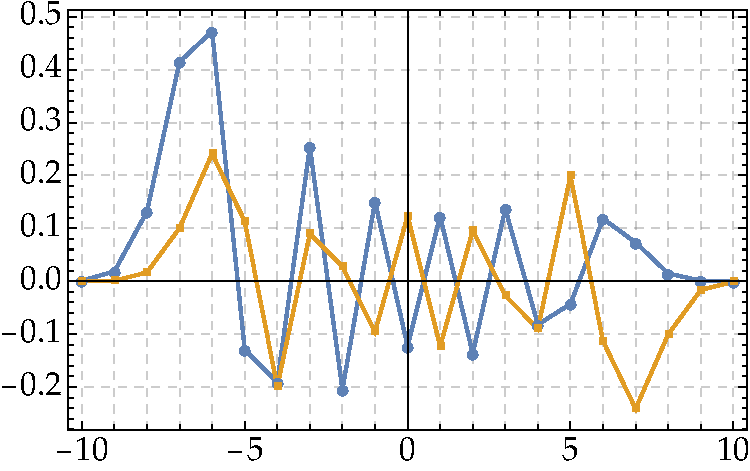
\includegraphics[width=\textwidth]{QW20steps_initstateUp}
        \begin{tikzpicture}
            \node (img) {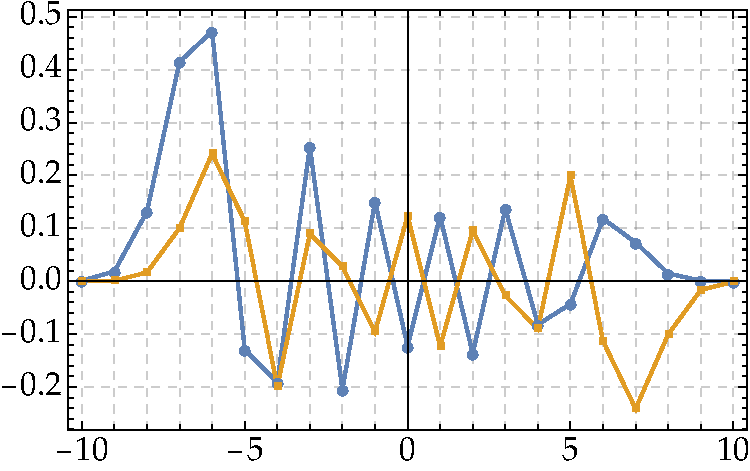
\includegraphics[width=0.9\textwidth]{QW20steps_initstateUp}};
            \node[below=of img, node distance=0cm, yshift=1cm,font=\small] {step number};
            \node[left=of img, node distance=0cm, rotate=90, anchor=center,yshift=-0.7cm,font=\small] {amplitude};
            \node at (0, 2.5) {\small\textbf{(a)} $20$ \emph{steps}};
        \end{tikzpicture}
    \end{subfigure}%
    \begin{subfigure}{0.5\textwidth}
        \centering
        % \caption{$40$ steps}
        % 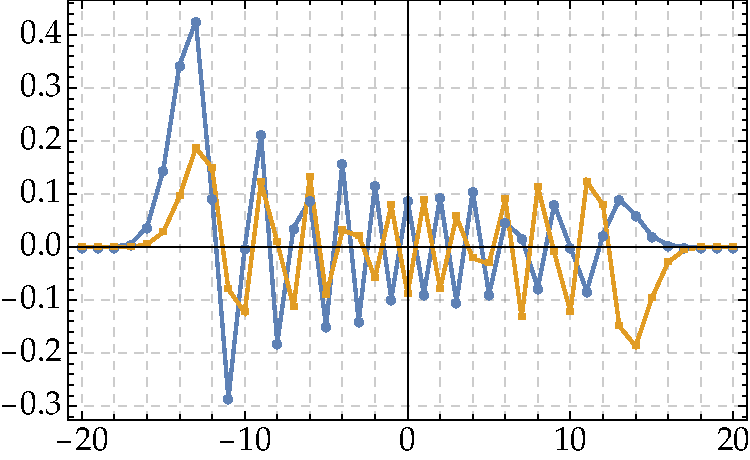
\includegraphics[width=\textwidth]{QW40steps_initstateUp}
        \begin{tikzpicture}
            \node (img) {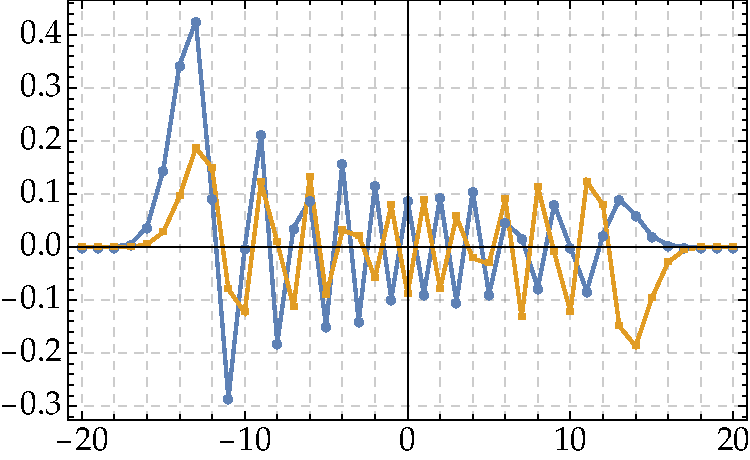
\includegraphics[width=0.9\textwidth]{QW40steps_initstateUp}};
            \node[below=of img, node distance=0cm, yshift=1cm,font=\small] {step number};
            \node at (0, 2.5) {\small\textbf{(a)} $40$ \emph{steps}};
        \end{tikzpicture}
    \end{subfigure}
    \caption{
        Output amplitudes after $20$ steps of Hadamard walk, with initial state $\ket{\Psi_0}\equiv\ket{\uparrow,0}$.
        Blue (circles) and orange (squares) points represent the output amplitudes corresponding to initial coin state $\ket\uparrow$ and $\ket\downarrow$, respectively.
    }
    \label{fig:intro:hadamardwalk_Nsteps2}
\end{figure}
% reindexForQW[amps_] := Transpose[
%    {{#[[1]], #[[2, 1]]}, {#[[1]], #[[2, 2]]}} & /@ 
%       Thread@{Range@Length@# - 1/2 - Length@#/2, #} &@amps
%    ];
% outAmps = 
%   QWEvolve[{1., 0}, ConstantArray[{\[Pi]/4, \[Pi]/2, \[Pi]/2}, 20], 
%     "SimulationMethod" -> "StepByStep"] // Partition[#, 2] &;
% fig = ListPlot[reindexForQW@outAmps, Joined -> True, 
%   PlotMarkers -> Automatic, Frame -> True, 
%   GridLines -> {Range[-20, 20], Range[-1, 1, 0.1]},
%   GridLinesStyle -> Directive[Opacity@.4, Gray, Dashed],
%   FrameStyle -> 
%    Directive[Black, FontFamily -> "TeX Gyre Pagella Math", 
%     FontSize -> 16]
%   ]

\tmpHeading{Single steps}
% As described in~\cref{sec:intro:QWs}, a single step of QW evolution consists of a \emph{coin flipping} operation, implemented through a unitary transformation $\calC$ applied to the coin, and a \emph{walking step}, in which the walker's state evolves conditionally to the state of the coin, through a controlled-shift operator $\calS$.
% We will denote with $\calHcoin$ and $\calHwalker$ the Hilbert spaces in which coin and walker states live, respectively.
% A general initial state $\ket\Psi\in\calHwalker\otimes\calHcoin$ can thus be written as
% \begin{equation}
% 	\ket\Psi \equiv \sum_{k=1}^n \sum_{s\in\{\uparrow,\downarrow\}}
% 	u_{k,s} \ket{k} \otimes \ket{s}.
% 	\label{eq:initial_state}
% \end{equation}
Assuming an initial state $\ket\Psi$ spanning $n$ walker positions, after one step we have
% After one step, this state evolves to
\begin{equation}
	\mathcal W_{\mathcal C} \ket\Psi \equiv
	\mathcal S \,\mathcal C \ket\Psi
	= \sum_{k=1}^n \sum_{s\in\{\uparrow,\downarrow\}}
	u_{k,s}
	\mathcal S \big( \ket{k} \otimes \mathcal C \ket{s} \big).
	\label{eq:QWs:step_operator_definition}
\end{equation}
% The controlled-shift operation is written here following the notation presented in~\cref{sec:intro:QWs}, and previously employed in~\cite{hoyer2009faster,montero2013unidirectional,montero2015quantum}: at each step, the walker either stands still or moves to the right, conditionally on whether the coin's state is $\ket{\uparrow}$ or $\ket{\downarrow}$ (cf.~\cref{fig:QWs:conceptual_scheme_walker})
% For two-dimensional coin states and initial states spanning a single position, the two formalism are equivalent, but our choice will allow for a tidier exposition and more efficient numerical simulations.

\begin{figure}[tb]
\center
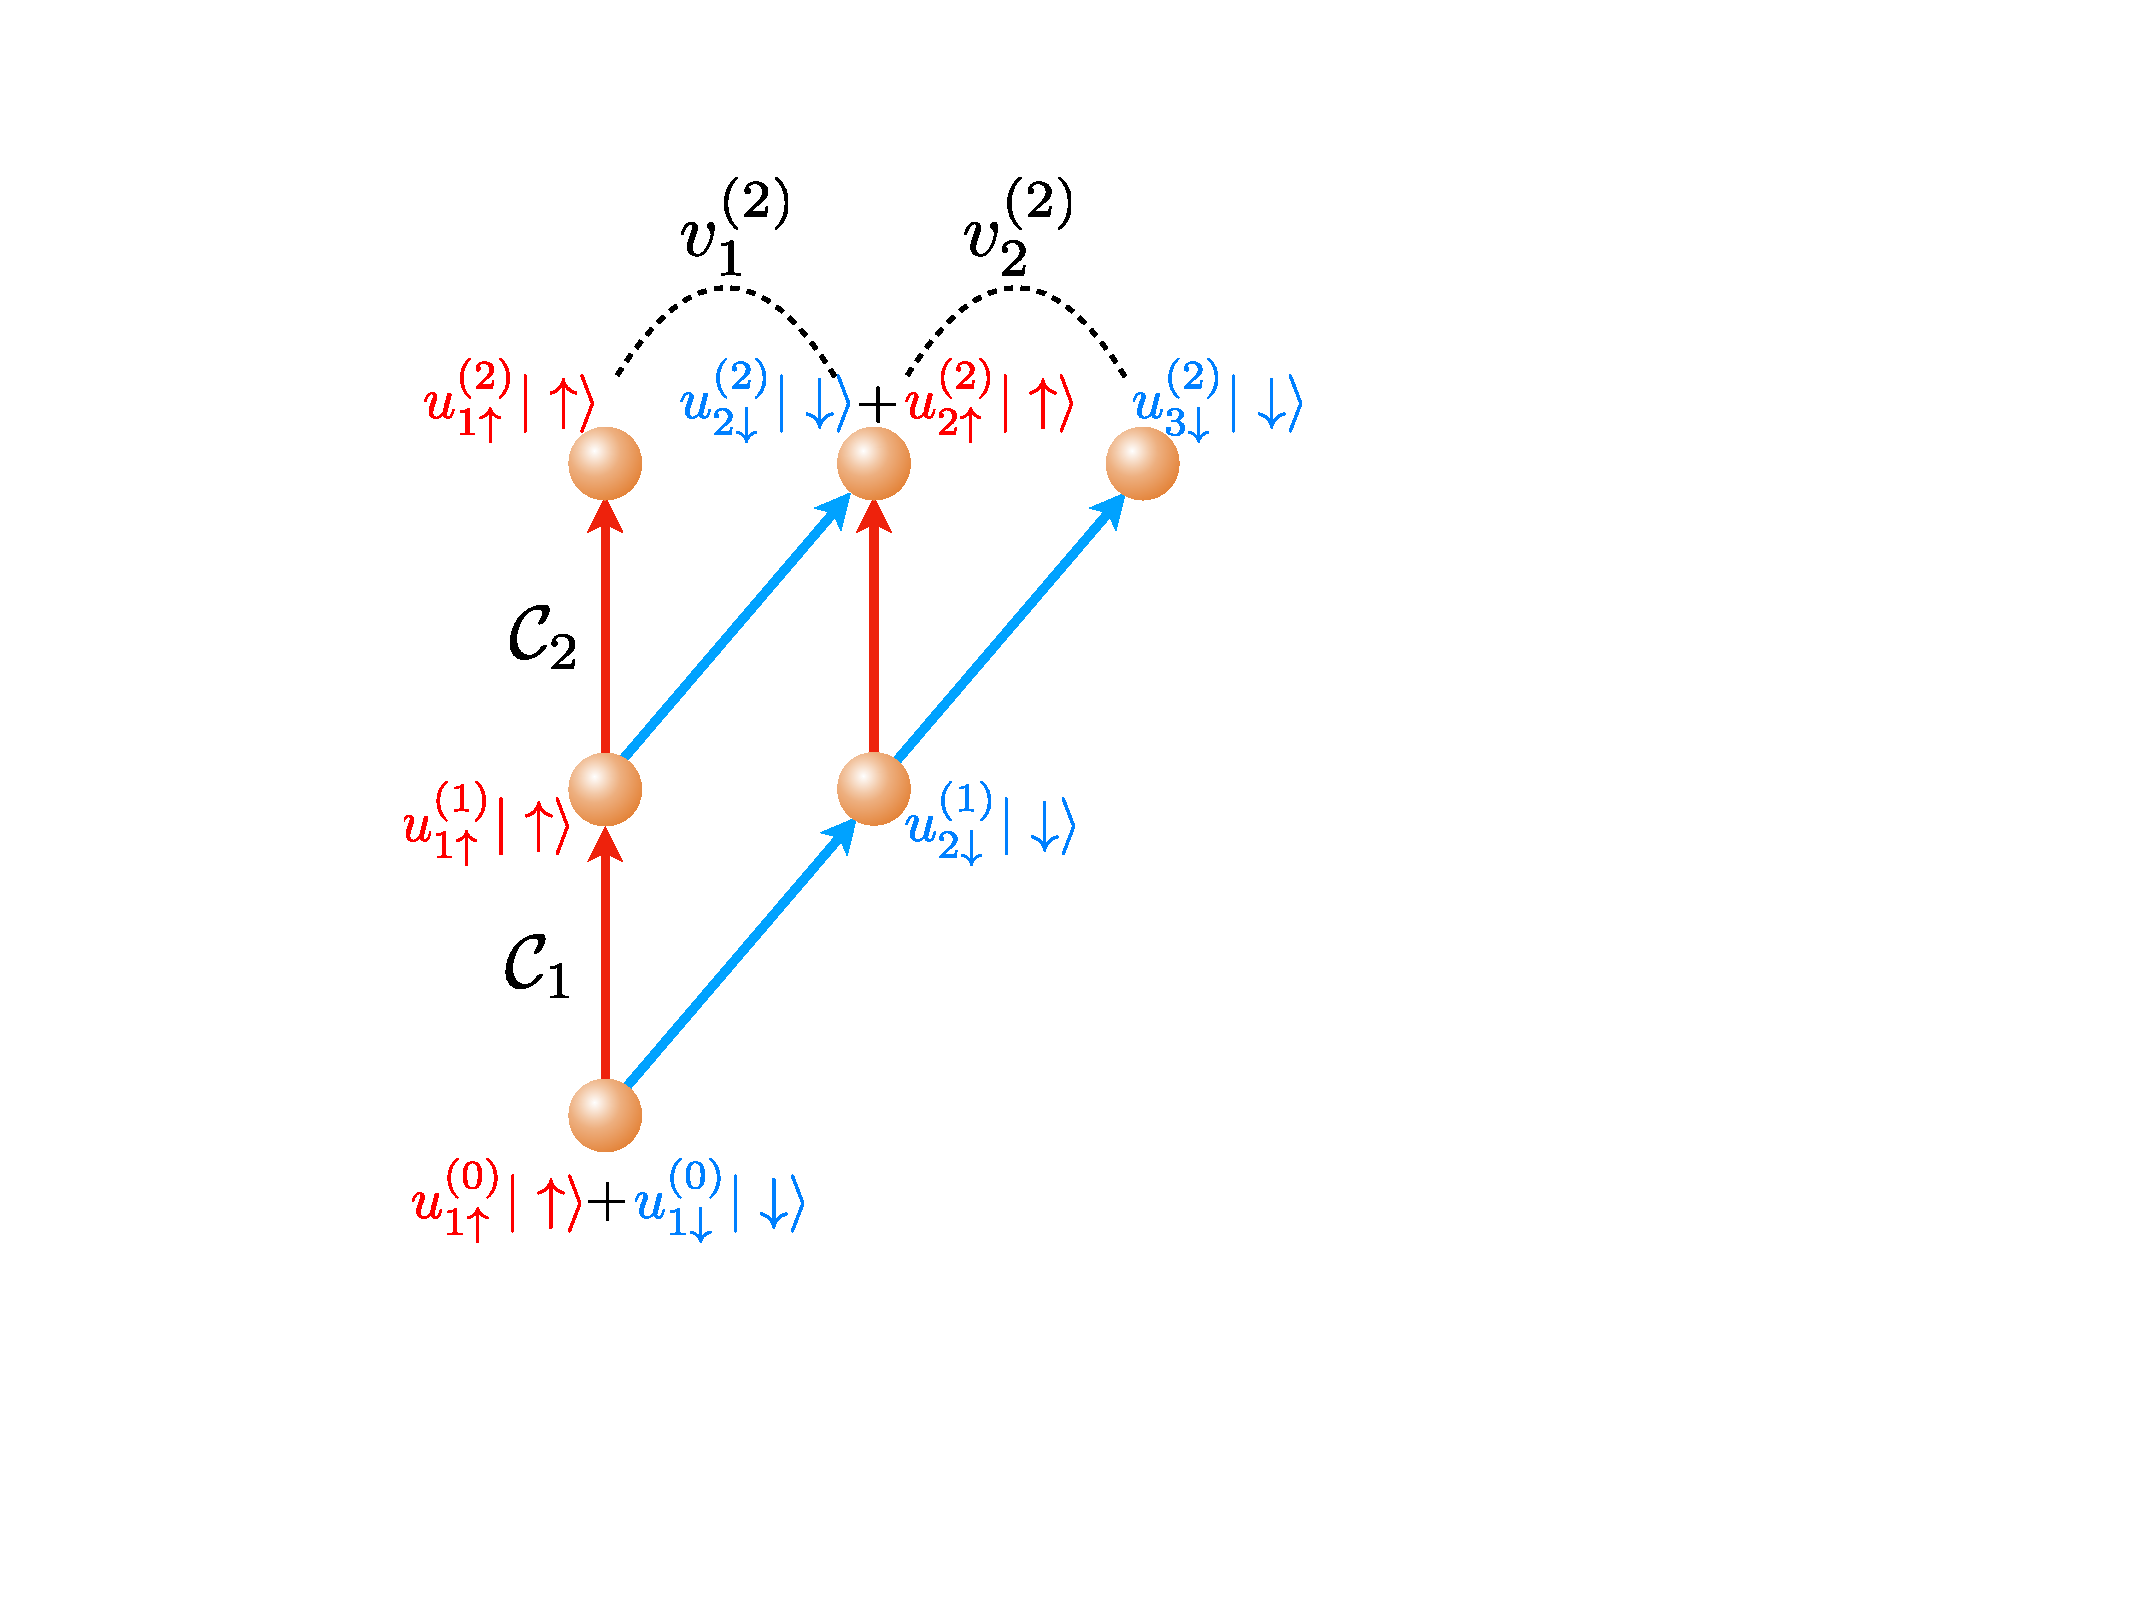
\includegraphics[width=0.3\columnwidth]{Scheme}
\caption{
    Schematic representation of how the amplitudes are distributed among the sites, at the various steps of the evolution.
    The red (blue) arrows represent the movement of the walker with coin state $\ket\uparrow$ ($\ket\downarrow$) after the coin flip.
    %It is clear from this representation why the ${u_{1,\downarrow} = u_{n+1, \uparrow} = 0}$ must hold.
    The coin operators $\mathcal C_i$ determine how the amplitude at each site is distributed between the red and blue arrows, and thus the two sites of the next layer with which it is connected.
    Here, $u_{i,s}^{(k)}$ denotes the amplitude at the $i$-th site, with coin state $\ket s$, after the $k$-th step.
    The vectors $\bs v_i$ are defined as
    $\bs v_1=(u_{1,\uparrow}^{(2)},u_{2,\downarrow}^{(2)})^T$ and
    $\bs v_2=(u_{2,\uparrow}^{(2)},u_{3,\downarrow}^{(2)})^T$.
    These vectors of amplitudes will prove useful to derive our results in~\cref{sec:QWs:2step_reachability}.
}
\label{fig:QWs:conceptual_scheme_walker}
\end{figure}

The explicit way $\calS$ and $\calW_\calC$ act on the basis states will prove useful in~\cref{sec:QWs:reachability_conditions}:
\begin{equation}
\begin{cases}
    \calS\ket{k,\uparrow} &= \ket{k,\uparrow}, \\
    \calS\ket{k,\downarrow} &= \ket{k+1, \downarrow},
\end{cases}
\qquad
\begin{cases}
    \calW_\calC\ket{k,\uparrow} &= c_{00} \ket{k,\uparrow} + c_{10} \ket{k+ 1,\downarrow}, \\
    \calW_\calC\ket{k,\downarrow} &= c_{01}\ket{k, \uparrow} + c_{11} \ket{k+1, \downarrow},
\end{cases}
\end{equation}
where we denoted the matrix elements of the coin operator as $(\calC)_{ij}=c_{ij}$.
We can write more concisely the combined action of $\calC$ and $\calS$ by focusing on how $\calW$ acts on the single sites.
To see this, suppose that $\ket{\Phi}=\calW_\calC\ket{\Phi'}$ for some $\ket{\Phi},\ket{\Phi'}$ and $\calC$.
Then,
\begin{equation}
    \begin{pmatrix}
        \braket{k,\uparrow}{\Phi} \\
        \braket{k + 1, \downarrow}{\Phi}
    \end{pmatrix} =
    \calC \begin{pmatrix}
        \braket{k,\uparrow}{\Phi'} \\
        \braket{k,\downarrow}{\Phi'}
    \end{pmatrix},
    \qquad \forall k=1,...,n.
    \label{eq:QWs:dynamics_on_single_positions}
\end{equation}
We will also make use of an alternative way to represent states in $\calHwalker\otimes\calHcoin$ spanning $n$ sites, via two-column matrices. We write each state as an $n\times 2$ matrix in which each row contains the amplitudes associated with the corresponding site, and each column the amplitudes associated with a coin state.
We thus write $\ket\Psi$ as the $n\times2$ matrix
\begin{equation}
    \ket\Psi\doteq \begin{pmatrix}
        \Psi_{1,\uparrow} & \Psi_{1,\downarrow} \\
        \Psi_{2,\uparrow} & \Psi_{2,\downarrow} \\
        \multicolumn{2}{c}{\vdots} \\ 
        \Psi_{n,\uparrow} & \Psi_{n,\downarrow} \\
    \end{pmatrix}.
    \label{eq:QWs:matrix_notation}
\end{equation}
In this notation, the coin operation only introduces coherence between amplitudes on the same row, while the shift $\calS$ acts by shifting the second column downwards.

\begin{examplebox}[label={ex:QWs:bimatrix_notation}]{QW evolution}
\fontsize{10pt}{10pt}\selectfont
    Here, we give explicit expressions for the states produced by a few steps of \ac{QW} evolution, using the matrix notation introduced in~\cref{eq:QWs:matrix_notation}. Let the initial state be $\ket{\Psi^{(0)}}\equiv\ket{1,\uparrow}$, and denote with $\calC_i$ be the coin operation at the $i$-th step, with elements $(\calC_i)_{jk}\equiv c^{(i)}_{jk}$.
    After a single step, we have
    \begin{equation}
        \ket{\Psi^{(1)}} =
        \begin{pmatrix}
            c^{(1)}_{11} & 0 \\
            0 & c^{(1)}_{21}
        \end{pmatrix}.
    \end{equation}
    After the second and third steps, we have
    \begin{equation}
        \ket{\Psi^{(2)}} =
        \begin{pmatrix}
            c^{(2)}_{11} c^{(1)}_{11} & 0 \\[0.4em]
            c^{(2)}_{12} c^{(1)}_{21} & c^{(2)}_{21} c^{(1)}_{11} \\[0.4em]
            0 & c^{(2)}_{22} c^{(1)}_{21} \\[0.4em]
        \end{pmatrix},
    \end{equation}
    \begin{equation}
        \ket{\Psi^{(3)}} =
        \begin{pmatrix}
            c^{(3)}_{11} c^{(2)}_{11} c^{(1)}_{11} & 0 \\[0.4em]
            c^{(3)}_{11} c^{(2)}_{12} c^{(1)}_{21} +
            c^{(3)}_{12} c^{(2)}_{21} c^{(1)}_{11} &
            c^{(3)}_{21} c^{(2)}_{11} c^{(1)}_{11} \\[0.4em]
            c^{(3)}_{12} c^{(2)}_{22} c^{(1)}_{21} &
            c^{(3)}_{21} c^{(2)}_{12} c^{(1)}_{21} +
            c^{(3)}_{22} c^{(2)}_{21} c^{(1)}_{11} \\[0.4em]
            0 & c^{(3)}_{22} c^{(2)}_{22} c^{(1)}_{21} \\[0.4em]
        \end{pmatrix}.
    \end{equation}
    While we do not give the explicit expressions for larger number of steps, we note how even from such few expressions a noticeable pattern emerges from the structure of the coefficients. For example, if we focus on the subscripts of each element of these matrices, and read them from the right to the left, we get the following expression:
    \begin{equation}
        \begin{pmatrix}
            (11)(11)(11) & 0 \\
            (11)(12)(21) + (12)(21)(11) & (11)(11)(12) \\
            (12)(22)(21) & (11)(12)(22) + (12)(21)(12) \\
            0 & (12)(22)(22)
        \end{pmatrix},
    \end{equation}
    where the ``$+$'' symbols is used here as a purely formal character, rather than as an actual sum. From this expression we can see how the following patterns emerge:
    \begin{itemize}
        \item Each sequence starts with a $1$ on the left, and ends with a $1$ for the first column, or with a $2$ for the second column. The fact that each column starts with a $1$ is due to the initial coin state being $\ket\uparrow$, and would have been a $2$ if we instead started with $\ket\downarrow$.
        \item Between each pair of integers, the middle numbers are always identical (e.g. we never have something like $(11)(21)$). This is because each pair $(ij)$ represents the matrix component of a corresponding step changing the coin state from $i$ to $j$.
        \item In each entry, the number of $2$s on the right component of each pair equals the number of steps forward that the walker. For example, in the third row, we always have exactly two pairs with a $2$ on the right, consistently with the third row corresponding to output states of the form $\ket{3,\alpha}$.
    \end{itemize}
    These observations tell us that the initial and final number in each sequence, as well as the elements in between each pair, are redundant. We can then represent the same state more efficiently by replacing each pair with its second element. We thus get
    \begin{equation}
        \begin{pmatrix}
            111 & 0 \\
            211 + 121 & 112 \\
            221 & 212 + 122 \\
            0 & 222
        \end{pmatrix}.
    \end{equation}
    This expression shows how finding the output amplitude corresponding to each one of the output modes is reduced to a purely combinatorial problem: starting with coin state $\ket\uparrow$ and evolving for $n$ steps, the output amplitude corresponding to the mode $\ket{k,s}$ with $s\in\{1,2\}$ has a number of contributions equal to the number of bit-strings of length $n$ that end with $s$ and have a number of $2$s equal to $k-1$.
    Once the set of bit-strings associated with a given output amplitude has been found, recovering the corresponding matrix elements of the coin operations, and thus the overall amplitude, is straightforward.

    As an example, suppose we are interested in knowing the amplitude associated with the walker evolving from $\ket{1,\uparrow}$ to $\ket{3,\downarrow}$ after $n=4$ steps. Following the above reasoning, we do not need to evolve the initial state through the associated unitary matrices, but can instead see directly that the amplitude is the one associated with the following four bit-strings:
    \begin{equation}
        1122, \quad 1212, \quad 2112,
    \end{equation}
    which are the possible bit-strings of four elements with two $2$s and ending with a $2$. The amplitude is therefore equal to
    \begin{equation}
        c^{(4)}_{22} c^{(3)}_{21} c^{(2)}_{11} c^{(1)}_{11} +
        c^{(4)}_{21} c^{(3)}_{12} c^{(2)}_{21} c^{(1)}_{11} +
        c^{(4)}_{21} c^{(3)}_{11} c^{(2)}_{12} c^{(1)}_{21}.
    \end{equation}
\end{examplebox}


\section{Analytical results}
\label{sec:QWs:reachability_conditions}

In this section we provide a complete characterisation of the output states of time-dependent discrete-time \acp{QW} on a line.
We will find that such a characterisation can be formulated in terms of a sequence of efficiently verifiable conditions on the amplitudes of the output state.
More precisely, given a candidate output state, these conditions allow to (1) verify whether there is a sequence of coin operations generating the target states after the prescribed number of steps, and (2) if the answer is positive, obtain a possible such sequence.

\subsection{One-step reachability condition}
\label{sec:QWs:1step_reachability}

Let us start by analysing what happens for small numbers of steps. This will help to get intuition into the more general result.

Suppose the walker is initially localised at the site $i=1$ with some unspecified initial coin state $\ket\alpha$.
% $\ket s=u_{1,\uparrow}^{(0)}\ket{1,\uparrow} + u_{1,\downarrow}^{(0)}\ket{1,\downarrow}$.
The initial state of the full system is then written as
\begin{equation}
    \ket*{\Psi^{(0)}} \equiv
    \ket1\otimes\ket\alpha \equiv
    \ket{1}\otimes \big(u^{(0)}_{1,\uparrow} \ket{\uparrow} +
    u^{(0)}_{1,\downarrow} \ket{\downarrow} \big),
\end{equation}
denoting with $u^{(0)}_{1,\uparrow},u^{(0)}_{1,\downarrow}$ the amplitudes of $\ket\alpha$.
Let $\calC_1$ denote the coin operation performed at the first step,
and let $\calW_{\calC_1}$ be the corresponding step operation.
The state after the first step is then
$\ket*{\Psi^{(1)}} \equiv \calW_{\calC_1} \ket*{\Psi^{(0)}}$.
Explicitly, this reads
\begin{equation}
    \ket*{\Psi^{(1)}} =
    \calS \ket1\otimes(\calC_1\ket\alpha) =
    \mel{\uparrow}{\calC_1}{\alpha} \ket{1,\uparrow} +
    \mel{\downarrow}{\calC_1}{\alpha} \ket{2,\downarrow}.
\end{equation}
A notable feature of this state is that there are two vanishing amplitudes:
\begin{equation}
    \braket*{1, \downarrow}{\Psi^{(1)}} = \braket*{2, \uparrow}{\Psi^{(1)}} = 0.
\end{equation}
Note how this feature is independent of the initial coin state $\ket\alpha$ or the coin operation $\calC_1$, but is rather a general property of states produced by this kind of \ac{QW} dynamic.
More generally, for any initial walker state $\ket{\Psi}$ spanning $n$ sites, the application of $\mathcal W_{\mathcal C_1}$ produces a state spanning $n+1$ sites and satisfying the equations
\begin{equation}
	\mel{1, \downarrow}{\mathcal W_{\mathcal C_1}}{\Psi} =
	\mel{n+1, \uparrow}{\mathcal W_{\mathcal C_1}}{\Psi} = 0.
	\label{eq:QWs:vanishing_endpoints}
\end{equation}
This is a direct consequence of the structure of $\calS$, and can also be understood graphically from the pictorial representation in~\cref{fig:QWs:conceptual_scheme_walker}.
Indeed, the action of $\calS$ on an arbitrary state
$\ket\Psi\equiv\sum_{k=1}^N \sum_s \Psi_{k,s}\ket{k,s}$ reads
\begin{equation}
    \calS\ket\Psi =
    \sum_{k=1}^N (\Psi_{k,\uparrow}\ket{k,\uparrow} + \Psi_{k,\downarrow}\ket{k+1,\downarrow}),
\end{equation}
which means that $\mel{1,\downarrow}{\calS}{\Psi}=\mel{N+1,\uparrow}{\calS}{\Psi}=0$.
We can restate this result using the matrix notation introduced in~\cref{eq:QWs:matrix_notation} by saying that all and only the states that are the output of a step of \ac{QW} evolution have the form
\begin{equation}
    \begin{pmatrix}
        \bullet & 0 \\
        \bullet & \bullet \\
        \multicolumn{2}{c}{\vdots} \\ 
        \bullet & \bullet \\
        0 & \bullet \\
    \end{pmatrix},
    \label{eq:QWs:matrix_notation_vanishing_endpoints}
\end{equation}
where the $\bullet$ represent arbitrary amplitudes.
The implication goes both ways: any state $\ket\Phi$ of a system spanning $n+1$ sites and with an additional spin-like degree of freedom such that
$
\braket{1, \downarrow}{\Phi} =
\braket{n+1, \uparrow}{\Phi} = 0
$,
is the output of one step of a QW evolution with suitable coin operator and initial coin state.
To see this, suppose there are a coin operation $\calC$ and a state $\ket{\Phi'}$ such that $\calW_\calC\ket{\Phi'}=\ket{\Phi}$.
We then see from~\cref{eq:QWs:dynamics_on_single_positions} that any $\calC$ can be used, with a corresponding initial state $\ket{\Phi'}$ given by
\begin{equation}
    \begin{pmatrix}
        \Phi'_{k,\uparrow} \\
        \Phi'_{k,\downarrow}
    \end{pmatrix} = \calC^{-1}
    \begin{pmatrix}
        \Phi_{k,\uparrow} \\
        \Phi_{k+1,\downarrow}
    \end{pmatrix}
\end{equation}
We conclude that any state $\ket\Phi$ satisfying $\Phi_{1,\downarrow}=\Phi_{n+1,\uparrow}=0$ can be produced by a single step of a QW evolution.

\subsection{Two-step reachability conditions}
\label{sec:QWs:2step_reachability}
We now consider the possible states after \textit{two} \ac{QW} steps.
Suppose $\ket\Psi$ spans $n+2$ modes and can be written as
$\ket\Psi=\calW_{\calC_2}\calW_{\calC_1}\ket*{\Psi^{(-2)}}$
for some unitaries $\calC_1,\calC_2$, and state $\ket*{\Psi^{(-2)}}$. We use the notation $\ket*{\Psi^{(-2)}}$ to remark this being a state obtained applying two ``inverse QW steps'' to $\ket*\Psi$.
We will show in this section that all such $\ket\Psi$ must satisfy a specific orthogonality condition on their amplitudes, and that this condition, paired with the one discussed in~\cref{sec:QWs:1step_reachability}, is sufficient to determine that a state $\ket\Psi$ is the output of two steps of some \ac{QW} dynamics.

From~\cref{sec:QWs:1step_reachability} we know that $\ket\Psi$ must be such that
$\Psi_{1,\downarrow}=\Psi_{n+2,\uparrow}=0$.
However, there is now an additional constraint to be taken into consideration. Namely, $\ket*{\Psi^{(-1)}}\equiv\calW_{\calC_1}\ket*{\Psi^{(-2)}}$ is also subject to the conditions derived in~\cref{sec:QWs:1step_reachability}:
$\Psi^{(-1)}_{1,\downarrow}=\Psi^{(-1)}_{n+1,\uparrow}=0$.
This constraint reflects on~\cref{eq:QWs:dynamics_on_single_positions}, which on the extremal sites now gives:
\begin{equation}
    \begin{pmatrix}
        \Psi_{1,\uparrow} \\
        \Psi_{2,\downarrow}
    \end{pmatrix} =
    \calC_1
    \begin{pmatrix}
        \Psi^{(-1)}_{1,\uparrow} \\
        \Psi^{(-1)}_{1,\downarrow}
    \end{pmatrix} =
    \calC_1
    \begin{pmatrix}
        \Psi^{(-1)}_{1,\uparrow} \\ 0
    \end{pmatrix},
\end{equation}
\begin{equation}
    \begin{pmatrix}
        \Psi_{n+1,\uparrow} \\
        \Psi_{n+2,\downarrow}
    \end{pmatrix} =
    \calC_1
    \begin{pmatrix}
        \Psi^{(-1)}_{n+1,\uparrow} \\
        \Psi^{(-1)}_{n+1,\downarrow}
    \end{pmatrix} =
    \calC_1
    \begin{pmatrix}
        0 \\
        \Psi^{(-1)}_{n+1,\downarrow}
    \end{pmatrix}.
\end{equation}
The unitarity of $\calC_1$ then directly implies that the length-$2$ vectors
$\begin{pmatrix}
    \Psi_{1,\uparrow} \\
    \Psi_{2,\downarrow}
\end{pmatrix}$
and
$\begin{pmatrix}
    \Psi_{n+1,\uparrow} \\
    \Psi_{n+2,\downarrow}
\end{pmatrix}$
are orthogonal.
This follows from the characterisation of unitaries as those matrices whose rows (equivalently, columns) form an orthonormal system for the underlying vector space.
Let us then define the vectors $\bs v_j$ as:
\begin{equation}
    \bs v_j \equiv \begin{pmatrix}
        \Psi_{j,\uparrow} \\ \Psi_{j+1,\downarrow}
    \end{pmatrix},
    \qquad
    \bs v_j^{(-k)} \equiv \begin{pmatrix}
        \Psi^{(-k)}_{j,\uparrow} \\ \Psi^{(-k)}_{j+1,\downarrow}
    \end{pmatrix}.
\end{equation}
The orthogonality condition characterising $\Psi$ becomes
$
    \bs v_1^\dagger \bs v_{n+1} \equiv \langle \bs v_1, \bs v_{n+1}\rangle = 0,
$
which, together with~\cref{sec:QWs:1step_reachability}, gives the following two explicit conditions:
% \begin{subequations}
% 	\begin{align}
% 		u^{(2)}_{1, \downarrow} = u^{(2)}_{3, \uparrow} = 0,
% 		\label{eq:vanishing_endpoints_after_2steps}\\
% 		u^{(2)*}_{1, \uparrow} u^{(2)}_{2, \uparrow}
% 		+ u^{(2)*}_{2, \downarrow} u^{(2)}_{3, \downarrow} = 0.
% 		\label{eq:1st_orthogonality_condition}
% 	\end{align}
% 	\label[pluralequation]{eq:both_2ndstep_conditions}
% \end{subequations}
\begin{subequations}
 	% \label[pluralequation]{eq:both_2ndstep_conditions}
    \label{eq:QWs:both_2ndstep_conditions}
    \begin{align}
        \Psi_{1,\downarrow} = \Psi_{n+2,\uparrow} = 0,
 		\label{eq:QWs:vanishing_endpoints_after_2steps}\\
        \Psi_{1,\uparrow}^* \Psi_{n+1,\uparrow} + 
        \Psi_{2,\downarrow}^* \Psi_{n+2,\downarrow} = 0.
 		\label{eq:QWs:1st_orthogonality_condition}
    \end{align}
\end{subequations}

Suppose now that $\ket\Phi$ is a state spanning $n+2$ sites and whose amplitudes satisfy~\cref{eq:QWs:both_2ndstep_conditions}.
Let $\ket*{\Phi^{(-1)}}$ be such that $\calW_{\calC_2}\ket*{\Phi^{(-1)}}$ for some $\calC_2$.
Then~\cref{eq:QWs:1st_orthogonality_condition} implies that
$(\Phi^{(-1)}_{1,\uparrow},\Phi^{(-1)}_{1,\downarrow})^T$
is orthogonal to
$(\Phi^{(-1)}_{n+1,\uparrow},\Phi^{(-1)}_{n+1,\downarrow})^T$.
However, we want $\ket\Phi$ to be the output of \textit{two} steps, which means that we need $\ket*{\Phi^{(-1)}}$ to be a viable output of a single step. As per our conclusions from given in~\cref{sec:QWs:1step_reachability}, $\ket*{\Phi^{(-1)}}$ must therefore have the form~\cref{eq:QWs:matrix_notation_vanishing_endpoints}, which then forces the coin $\calC_2$ to be such that
\begin{equation}
    \begin{pmatrix}
        \Psi_{1,\uparrow} \\ \Psi_{2,\downarrow}
    \end{pmatrix} =
    \calC_2 \begin{pmatrix}
        a \\ 0
    \end{pmatrix},
    \qquad
    \begin{pmatrix}
        \Psi_{n,\uparrow} \\ \Psi_{n+1,\downarrow}
    \end{pmatrix} =
    \calC_2 \begin{pmatrix}
        0 \\ b
    \end{pmatrix}.
\end{equation}
Basic linear algebra then tells us that $\calC_2$ should have the form
\begin{equation}
    \calC_2 = \begin{pmatrix}
        N_1 \Psi_{1,\uparrow} & N_2 e^{i\theta} \Psi_{n,\uparrow} \\
        N_1 \Psi_{2,\downarrow} & N_2 e^{i\theta} \Psi_{n+1,\downarrow}
    \end{pmatrix},
    \label{eq:QWs:coin_twosteps}
\end{equation}
where $N_1, N_2$ are constants needed to make the columns normalised, and $\theta\in\RR$ is an arbitrary phase.
It is worth noting that an additional phase factor could be added to the first column, but this would not make any difference, as it would amount to a global phase added to the unitary. In other words,~\cref{eq:QWs:coin_twosteps} determines an element of $\mathbf{U}(2)$ only up to its determinant\footnote{A more precise version of this statement is to say that we are determining the coins as elements of the quotient space $\mathbf{U}(2)/\mathbf U(1)\simeq\mathbf{SU}(2)$, in which matrices differing only by a multiplicative phase (equivalently, unitaries with different determinants), are considered as identical.}.
This choice of $\calC_2$ makes $\ket*{\Phi^{(-1)}}=\calW_{\calC_2}^{-1}\ket\Phi$ a possible outcome of a single step of \ac{QW} evolution.
Then, as per~\cref{sec:QWs:1step_reachability}, for any choice of $\calC_1$ we have that
$\calW_{\calC_1}^{-1}\calW_{\calC_2}^{-1}\ket\Phi$
is a state which after two steps produces the target $\ket\Phi$.


\subsection{Three-step reachability conditions}
\label{sec:QWs:3step_reachability}
Let us now consider an output of three steps:
$\ket*{\Psi} \equiv \calW_{\calC_3}\calW_{\calC_2}\calW_{\calC_1} \ket*{\Psi^{(-3)}}$,
and assume that this state occupies $n+3$ position modes.
Then, denoting with
$\ket*{\Psi^{(-1)}} \equiv \calW_{\calC_2}\calW_{\calC_1} \ket*{\Psi^{(-3)}}$
the state at the previous step, we have that the amplitudes of $\ket*{\Psi^{(-1)}}$ must satisfy~\cref{eq:QWs:both_2ndstep_conditions}.
Here, these conditions have the form
$\bs v_1^{\dagger(-1)} \bs v_{n+1}^{(-1)}=0$,
which can be rewritten as
\begin{equation}
\begin{gathered}
	0 = \bs v_1^{\dagger(-1)} \bs v_{n+1}^{(-1)} = 
	\begin{pmatrix} \Psi^{(-1)*}_{1,\uparrow} & \Psi^{(-1)*}_{2,\downarrow} \end{pmatrix}
	\begin{pmatrix} \Psi^{(-1)}_{n+1,\uparrow} \\ \Psi^{(-1)}_{n+2,\downarrow} \end{pmatrix}
	\\
	=
	\begin{pmatrix} \Psi^{(-1)*}_{1,\uparrow} & \Psi^{(-1)*}_{1,\downarrow} \end{pmatrix}
	\begin{pmatrix} \Psi^{(-1)}_{n+1,\uparrow} \\ \Psi^{(-1)}_{n+1,\downarrow} \end{pmatrix} +
	\begin{pmatrix} \Psi^{(-1)*}_{2,\uparrow} & \Psi^{(-1)*}_{2,\downarrow} \end{pmatrix}
	\begin{pmatrix} \Psi^{(-1)}_{n+2,\uparrow} \\ \Psi^{(-1)}_{n+2,\downarrow} \end{pmatrix},
\end{gathered}
\end{equation}
where we used
$\Psi^{(-1)}_{1,\downarrow} = \Psi^{(-1)}_{n+2,\uparrow} = 0$.
Applying \cref{eq:QWs:dynamics_on_single_positions} on the above we get
\begin{equation}
\begin{aligned}
    \bs v_1^{\dagger} \calC_3 \calC_3^\dagger \bs v_{n+1}+
    \bs v_2^{\dagger} \calC_3 \calC_3^\dagger \bs v_{n+2}  =
    \bs v_1^{\dagger} \bs v_{n+1} +
    \bs v_2^{\dagger} \bs v_{n+2} = 0.
\end{aligned}
\label{eq:QWs:last_condition_for_psi3}
\end{equation}
Following a reasoning similar to the one used in the previous section, we conclude that the amplitudes of $\ket*{\Psi}$ satisfy three conditions:
the vanishing of the extremal amplitudes, $\bs v_1^{\dagger} \bs v_{n+2} = 0$, and~\cref{eq:QWs:last_condition_for_psi3}.

\subsection{Generalised reachability conditions}
\label{sec:QWs:general_reachability_conditions}

We analyse here the generalisation of the conditions derived in~\cref{sec:QWs:1step_reachability,sec:QWs:2step_reachability,sec:QWs:3step_reachability}, giving the conditions characterising states that can be the output of $m$ steps of some time-dependent QW.

Let $\ket\Psi$ be a state spanning $n+m$ sites, which is the output of at least $m$ steps of \ac{QW} evolution, so that
\begin{equation}
	\ket\Psi =
	\calW_{\calC_{m}} \calW_{\calC_{m-1}} ... \calW_{\calC_{1}}
    \ket{\Psi^{(-m)}},
	\label{eq:QWs:starting_point}
\end{equation}
for some set of coin operators $\{\calC_i \}$ and initial state $\ket{\Psi^{(-m)}}$.
Here, $\ket{\Psi^{(-m)}}$ is an arbitrary state spanning $n$ positions (and which in particular is not required to satisfy any reachability condition of its own).
We want to show that, for any set of coin operators $\{\calC_i \}$, \cref{eq:QWs:starting_point} implies that $\ket\Psi$ satisfies the following conditions:
% \begin{equation}
\begin{gather}
	\Psi_{1,\downarrow} = \Psi_{n+m, \uparrow} = 0,
    \label{eq:QWs:vanishing_amplitudes}
	\\
    \sum_{i=1}^s \bs v_i^\dagger \bs v_{m+(n-1)-s+i} = 0,
	\text{ for } s=1,\ldots, m-1,
	\label{eq:QWs:orthogonality_conditions_for_vs}
\end{gather}
where $\bs v_{i}$ is again defined as
% \begin{equation*}
% 	\bs v_i \equiv
% 	\begin{pmatrix}
% 		\Psi_{i,\uparrow} \\ \Psi_{i+1, \downarrow}
% 	\end{pmatrix}.
% \end{equation*}
% \end{equation}
$\bs v_i \equiv (\Psi_{i,\uparrow}, \Psi_{i+1, \downarrow})^T$.
The cases $m=2$ and $m=3$ were worked out in~\cref{sec:QWs:2step_reachability,sec:QWs:3step_reachability},
so let us assume the statement to be true for $m$ and show that this implies it for $m+1$.
The main idea is to see how each one of the equations in \cref{eq:QWs:orthogonality_conditions_for_vs} transforms after one step.
Denote the amplitudes after a single step with $\Psi'_{i,\alpha}$.
The relation between primed and unprimed amplitudes is then
\begin{equation}
	\bs v_i^\prime
	= \mathcal C
	\begin{pmatrix}
		\Psi_{i,\uparrow} \\ \Psi_{i, \downarrow}
	\end{pmatrix},
	\text{ for each }
	i = 1, \dots, m,
	% \label{eq:evolution_amplitudes}
\end{equation}
for some unitary $\calC$,
where $\bs v'_i \equiv (\Psi_{i,\uparrow}',\Psi_{i+1,\downarrow}')^T$.
In~\cref{fig:QWs:visualisation_PsiVsPsip} we show schematically how the amplitudes of a state $\ket\Psi$ are related with the amplitudes of $\calW_\calC\ket\Psi$.
This directly implies, for all $i, j$,
\begin{equation}
	\begin{pmatrix}
		\Psi^*_{i, \uparrow} & \Psi^*_{i, \downarrow}
	\end{pmatrix}
	\begin{pmatrix}
		\Psi_{j, \uparrow} \\ \Psi_{j, \downarrow}
	\end{pmatrix}
	=
	\bs v^{\prime\dagger}_{i} \cdot \bs v^\prime_j.
    \label{eq:QWs:transition_us_to_vprimes}
\end{equation}
Explicitly, the $s$-th term in \cref{eq:QWs:orthogonality_conditions_for_vs} reads
\begin{equation}
	\bs v_1^\dagger \bs v_{m+n-s}
	+ \bs v_2^\dagger \bs v_{m+n-s+1}
	+ ...
	+ \bs v_{s-1}^\dagger \bs v_{m+n-2}
    + \bs v_s^\dagger \bs v_{m+n-1} = 0.
\end{equation}
Rewriting the LHS in terms of the amplitudes, rearranging the terms, and remembering that $\Psi_{1, \downarrow} = \Psi_{m+n, \uparrow} = 0$, we get
\begin{equation}
\begin{aligned}
	\begin{pmatrix}
		\Psi^*_{1, \uparrow} & \Psi^*_{1, \downarrow}
	\end{pmatrix}
	\begin{pmatrix}
		\Psi_{m+n-s, \uparrow} \\ \Psi_{m+n-s, \downarrow}
	\end{pmatrix}
	+
	\begin{pmatrix}
		\Psi^*_{2, \uparrow} & \Psi^*_{2, \downarrow}
	\end{pmatrix}
	\begin{pmatrix}
		\Psi_{m+n-s+1, \uparrow} \\ \Psi_{m+n-s+1, \downarrow}
	\end{pmatrix} + \dots\\
	+ 
	\begin{pmatrix}
		\Psi^*_{s, \uparrow} & \Psi^*_{s, \downarrow}
	\end{pmatrix}
	\begin{pmatrix}
		\Psi_{m+n-1, \uparrow} \\ \Psi_{m+n-1, \downarrow}
	\end{pmatrix}
	+
	\begin{pmatrix}
		\Psi^*_{s+1, \uparrow} & \Psi^*_{s+1, \downarrow}
	\end{pmatrix}
	\begin{pmatrix}
		\Psi_{m+n, \uparrow} \\ \Psi_{m+n, \downarrow}
	\end{pmatrix} = 0.
\end{aligned}
\end{equation}
Using \cref{eq:QWs:transition_us_to_vprimes} we then get
\begin{equation}
	\bs v^{\prime\dagger}_1 \bs v^\prime_{m+n-s} +
	\bs v^{\prime\dagger}_2 \bs v^\prime_{m+n-s+1} +
	... +
    \bs v^{\prime\dagger}_{s} \bs v^\prime_{m+n-1} +
	\bs v^{\prime\dagger}_{s+1} \bs v^\prime_{m+n} = 0,
\end{equation}
or, equivalently,
$\displaystyle \sum_{i=1}^{s+1} \bs v^{\prime\dagger}_i \bs v^\prime_{m+n-(s+1)+i}=0$
for $s=1,\dots,m-1$.

\begin{figure}[tb]
    \centering
    \begin{equation}\scalebox{0.8}{$
    \begin{pmatrix}
    \textcolor[rgb]{0.82,0.01,0.11}{\Psi_{1,\uparrow}} & 0 \\
    \textcolor[rgb]{0.96,0.65,0.14}{\Psi_{2,\uparrow}} &
    \textcolor[rgb]{0.96,0.65,0.14}{\Psi_{2,\downarrow}} \\
    \textcolor[rgb]{0.55,0.34,0.16}{\Psi_{3,\uparrow}} &
    \textcolor[rgb]{0.55,0.34,0.16}{\Psi_{3,\downarrow}} \\
    \vdots  & \vdots \\
    \textcolor[rgb]{0.25,0.46,0.02}{\Psi_{m+n-1,\uparrow}} &
    \textcolor[rgb]{0.25,0.46,0.02}{\Psi_{m+n-1,\downarrow}} \\
    0 & \textcolor[rgb]{0.56,0.07,1}{\Psi_{m+n,\downarrow}} \\
    0 & 0
    \end{pmatrix}
    \rightarrow
    \begin{pmatrix}
    \textcolor[rgb]{0.82,0.01,0.11}{\Psi'_{1,\uparrow}} & 0 \\
    \textcolor[rgb]{0.96,0.65,0.14}{\Psi'_{2,\uparrow}} &
    \textcolor[rgb]{0.82,0.01,0.11}{\Psi'_{2,\downarrow}} \\
    \vdots &
    \textcolor[rgb]{0.96,0.65,0.14}{\Psi'_{3,\downarrow}} \\
    \vdots & \vdots \\
    \textcolor[rgb]{0.25,0.46,0.02}{\Psi'_{m+n-1,\uparrow}} & \vdots \\
    \textcolor[rgb]{0.56,0.07,1}{\Psi'_{m+n,\uparrow}} &
    \textcolor[rgb]{0.25,0.46,0.02}{\Psi'_{m+n,\downarrow}}\\
    0 & \textcolor[rgb]{0.56,0.07,1}{\Psi'_{m+n+1,\downarrow}}
    \end{pmatrix}$}
    \end{equation}
    \caption{
        Relation between $\ket\Psi$ and $\ket{\Psi'}\equiv\calW_\calC\ket\Psi$ as used in~\cref{sec:QWs:general_reachability_conditions}. The different colors correspond to pairs of amplitudes connected via $\calC$, as per~\cref{eq:QWs:dynamics_on_single_positions}.
    }
    \label{fig:QWs:visualisation_PsiVsPsip}
\end{figure}

This proves that, given $\ket\Psi$ satisfying~\cref{eq:QWs:orthogonality_conditions_for_vs}, any state of the form $\ket{\Psi'}=\calW_\calC\ket\Psi$ satisfies the $m-1$ constraints:
\begin{equation}
    \sum_{i=1}^{s} \bs v^{\prime\dagger}_i \bs v^\prime_{(m+1)+(n-1)-s+i}=0
	\text{ for }
	s = 2,...,m,
	\label{eq:QWs:general_orthogonality_almost_finished}
\end{equation}
which we can recognise as equivalent to~\cref{eq:QWs:orthogonality_conditions_for_vs} with $m\to m+1$, except for the $s=1$ condition, which amounts to $\bs v_1^{\prime\dagger}\bs v'_{(m+1)+n-1}=0$.
This last condition follows from $\Psi_{1,\downarrow}=\Psi_{n+m,\uparrow}=0$, as shown in~\cref{sec:QWs:2step_reachability}, and thus the induction step is completed.

In the special case of the initial state spanning a single position,~\cref{eq:QWs:orthogonality_conditions_for_vs} tells us that if a state $\ket{\Psi}$ is the output of $n$ steps with some initial state $\ket{1,\alpha}$, then $\Psi_{1,\downarrow}=\Psi_{n+1,\uparrow}=0$, and the following $n-1$ conditions are met:
\begin{equation}
    \sum_{i=1}^s \bs v_i^{\dagger} \bs v_{n-s+i} = 0,
    \text{ for every } s=1,..,n-1.
    \label{eq:QWs:general_reachability_conditions}
\end{equation}

\begin{table}[tbh]
\centering
\scalebox{0.8}{
\begin{tabular}{cc@{\quad}l}
    \toprule
    \textbf{State} & \textbf{Occupied sites} & \textbf{Constraints} \\
    \midrule \\
    $\ket*{\Psi^{(0)}}$ & 1 & none \\
    \addlinespace[2pt]
    $\ket*{\Psi^{(1)}}$ & 2 & $u_{1,\downarrow} = u_{2,\uparrow} = 0$ \\
    \addlinespace[5pt]
    $\ket*{\Psi^{(2)}}$ & 3 &
    $\begin{dcases}
        u_{1,\downarrow} = u_{3,\uparrow} = 0 \\
        \bs v_1^{\dagger} \bs v_2 = 0
    \end{dcases}$ \\
    \addlinespace[5pt]
    % \addlinespace[0pt]\\
    $\ket*{\Psi^{(3)}}$ & 4 &
    $\begin{dcases}
        u_{1,\downarrow} = u_{4,\uparrow} = 0 \\
        \bs v_1^{\dagger} \bs v_3 = 0 \\
        \bs v_1^{\dagger} \bs v_2 + \bs v_2^{\dagger} \bs v_3 = 0
    \end{dcases}$ \\\addlinespace[4pt]
    $\vdots$ & $\vdots$ & \qquad\quad$\vdots$ \\
    $\ket*{\Psi^{(n)}}$ & $n$+1 &
    $\begin{dcases}
        u_{1,\downarrow} = u_{n + 1,\uparrow} = 0 \\
        \sum_{i=1}^s \bs v_i^{\dagger} \bs v_{n-s+i} = 0
    \end{dcases}$ \\
    \bottomrule
\end{tabular}
}
\caption{
    Summary of the conditions characterising the states at the various stages of the evolution.
    For better clarity, we have avoided the use of superscripts on the amplitudes.
The amplitudes in each row refer to the corresponding state at that step.
    The conditions shown in the case $\ket*{\Psi^{(n)}}$ hold for all $s=1,..., n-1$, consistently with~\cref{eq:QWs:general_reachability_conditions}.
}
\label{table:QWs:constraints}
\end{table}

\begin{examplebox}[label=ex:QWs:conditions_few_steps]{Example of application of reachability conditions}
\fontsize{10pt}{10pt}\selectfont
    To illustrate how the derived conditions work, consider an example with initial state
    \begin{equation}
        \ket{\Psi} = \frac{1}{\sqrt4} (
        \ket{1,0} + \ket{2,+} + \ket{3, -} + \ket{4, 1}
        ).
    \end{equation}
    Let $\calC_1=H$, with $H$ the Hadamard matrix, which satisfies
    \begin{equation}
        H\ket0=\ket+, \quad H\ket1=\ket-,
        \quad H\ket+=\ket0, \quad H\ket-=\ket1.
    \end{equation}
    Following the matrix notation introduced in~\cref{eq:QWs:matrix_notation}, we have
    \begin{equation}
        \ket{\Psi} =
        \frac{1}{\sqrt4}
        \begin{pmatrix}
            1 & 0 \\
            1/\sqrt2 & 1/\sqrt2 \\
            1/\sqrt2 & -1/\sqrt2 \\
            0 & 1
        \end{pmatrix}.
    \end{equation}
    As this state satisfies the conditions given in~\cref{sec:QWs:1step_reachability} about the vanishing endpoints, $\Psi_{1,\downarrow}=\Psi_{4,\uparrow}=0$, we know that this is a possible output of a single step. On the other hand, it does not satisfy the conditions in~\cref{sec:QWs:2step_reachability} to be the output of \textit{two} steps.
    Consider now the evolved state $\ket*{\Psi^{(1)}}\equiv\calW_{\calC_1}\ket\Psi$ with $\calC_1\equiv H\equiv\frac{1}{\sqrt2}(I+Z)$ the Hadamard matrix. In matrix notation, this will be
    \begin{equation}
        \ket*{\Psi^{(1)}} =
        \frac{1}{\sqrt4}
        \begin{pmatrix}
            1/\sqrt2 & 0 \\
            1 & 1/\sqrt2 \\ 
            0 & 0 \\
            1/\sqrt2 & 1 \\
            0 & -1/\sqrt2
        \end{pmatrix}.
        \label{eq:QWs:example_psi'}
    \end{equation}
    The vectors $\bs v^{(1)}$ then equal $\bs v^{(1)}_1=(1/\sqrt2, 1/\sqrt2)$ and
    $\bs v^{(1)}_4=(1/\sqrt2, -1/\sqrt2)$,
    which are orthogonal, consistently with $\ket*{\Psi^{(1)}}$ being output of two steps.
    Let us consider an additional step with coin $\calC_2=\frac{1}{\sqrt2}(I + iX)$.
    Writing the output with $\ket*{\Psi^{(2)}}=\calW_{\calC_2}\ket*{\Psi^{(1)}}$, we have
    \begin{equation}
        \ket*{\Psi^{(2)}} = \frac{1}{4}
        \begin{pmatrix}
            1 & 0 \\
            i + \sqrt2 & i \\
            0 & 1 + i\sqrt2 \\
            1 + i\sqrt2 & 0 \\
            -i & i + \sqrt2 \\
            0 & -1
        \end{pmatrix}.
    \end{equation}
    The relevant $\bs v^{(2)}$ vectors are
    \begin{equation}
    \begin{aligned}
        \bs v^{(2)}_1 = \frac{1}{4}\begin{pmatrix} 1 \\ i \end{pmatrix},
        \,\,
        \bs v^{(2)}_2 = \frac{1}{4}\begin{pmatrix} \sqrt2 + i \\ 1 + i\sqrt2 \end{pmatrix},
        \,\,
        \bs v^{(2)}_4 = \frac{1}{4}\begin{pmatrix} 1 + i\sqrt2\\ \sqrt2 + i \end{pmatrix},
        \,\,
        \bs v^{(2)}_5 = \frac{1}{4}\begin{pmatrix} -i \\ -1 \end{pmatrix},
    \end{aligned}
    \end{equation}
    It is then straightforward to verify that
    $\bs v_1^{(2)\dagger}\bs v_5^{(2)} = 0$.
    Furthermore,
    $\bs v_1^{(2)\dagger}\bs v_4^{(2)} = 1/8$
    and $\bs v_2^{(2)\dagger}\bs v_5^{(2)} = -1/8$,
    thus 
    $\bs v_1^{(2)\dagger}\bs v_4^{(2)} + \bs v_2^{(2)\dagger}\bs v_5^{(2)} = 0$,
    again consistently with the results of~\cref{sec:QWs:3step_reachability}.
    As a last remark, let us show how we would go in recovering the coin operators generating $\ket*{\Psi^{(2)}}$, assuming we are only given this state without further knowledge.
    The idea behind such reconstruction is to observe that if $\tilde\calC_1$ is such that $\calW_{\tilde\calC_1}\ket{\Phi'}=\ket*{\Psi^{(2)}}$ for some $\ket{\Phi'}$, then, from~\cref{eq:QWs:dynamics_on_single_positions}, we know that $\tilde\calC_1^\dagger \bs v_1^{(2)}\simeq(1,0)^T$ and $\tilde\calC_1^\dagger \bs v_5^{(2)}\simeq(0,e^{i\phi})^T$ for some $\phi_1\in\RR$. It follows that
    \begin{equation}
        \tilde\calC_1 =
        \frac{1}{\sqrt2} \begin{pmatrix}
            1 & e^{i\phi_1}i \\
            i & e^{i\phi_1}\phantom{1}
        \end{pmatrix}.
    \end{equation}
    This is clearly consistent with the coin operation being $\frac{1}{\sqrt2}(I+iX)$, but also shows that multiple initial states are compatible with the output, thanks to the freedom in choosing $\phi_1$. The corresponding $\ket{\Phi'}$ are then
    \begin{equation}
        \ket{\Phi'} = \frac{1}{2\sqrt2}
        \begin{pmatrix}
            1 & 0 \\
            \sqrt2 & e^{-i\phi_1} \\
            0 & 0 \\
            1 & \sqrt2 e^{-i\phi_1} \\
            0 & -e^{-i\phi_1}
        \end{pmatrix},
    \end{equation}
    consistently with~\cref{eq:QWs:example_psi'}.
    Going further back, we use $\sqrt2\bs v_1^{(1)}=(1,e^{-i\phi_1})^T$ and $\sqrt2\bs v_4^{(1)}=(1,-e^{-i\phi_1})^T$ to find the previous possible coins $\tilde\calC_2$ to be of the form
    \begin{equation}
        \tilde\calC_2 = \frac{1}{\sqrt2} \begin{pmatrix}
            1 & e^{i\phi_2} \\
            e^{-i\phi_1} & -e^{i(\phi_2-\phi_1)}
        \end{pmatrix},
    \end{equation}
    for all $\phi_2\in\RR$. The reconstructed initial state $\ket\Phi$ is then found to have the form
    \begin{equation}
        \ket\Phi = \frac{1}{2\sqrt2}
        \begin{pmatrix}
            \sqrt2 & 0 \\
            1 & e^{-i\phi_2} \\
            1 & -e^{-i\phi_2} \\
            0 & \sqrt2 e^{-i\phi_2}
        \end{pmatrix}.
    \end{equation}
    An interesting feature emerging from this example is that the freedom in the choice of the coin operations does not ``cumulate'', in the sense that the possible states producing a target after a number of steps are still uniquely defined up to only a phase difference between the two coin states.
\end{examplebox}

\subsection{Find coin operators generating a state}
\label{sec:QWs:coin_operators_generating_state}

\tmpHeading{Goal of the section}
In~\cref{sec:QWs:reachability_conditions} we showed that, if $\ket\Psi=\calW_{\calC_n}\cdots\calW_{\calC_1}\ket{\Psi_{\on{in}}}$, then the amplitudes of $\ket\Psi$ must satisfy the conditions given in~\cref{eq:QWs:general_reachability_conditions}.
Here we show that also the opposite holds: given a state $\ket\Psi$ satisfying~\cref{eq:QWs:general_reachability_conditions}, there is always a choice of coin operations $\calC_i$ and initial state $\ket{\Psi_{\on{in}}}$ that produce $\ket\Psi$.

\tmpHeading{Vanishing amplitudes imply state is output of one step}
Suppose that a state $\ket\Psi$ over $n$ sites satisfies $\Psi_{1,\downarrow}=\Psi_{n,\uparrow}=0$. Then, for any choice of unitary coin operator $\calC$, there is some $\ket*{\Psi^{(-1)}}$ such that $\ket\Psi=\calW_\calC\ket*{\Psi^{(-1)}}$.
This is straightforward, as $\calW_\calC\ket*{\Psi^{(-1)}}$ will always have vanishing extremal amplitudes, regardless of $\calC$. For a given choice of $\calC$, the initial state $\ket*{\Psi^{(-1)}}$ is uniquely determined by $\ket*{\Psi^{(-1)}}=\calW_\calC^{-1}\ket\Psi$.

\tmpHeading{Reconstructing coin operators after \emph{two} steps}
Suppose now that $\ket\Psi$, on top of $\Psi_{1,\downarrow}=\Psi_{n,\uparrow}=0$, also satisfies $\bs v_1^\dagger \bs v_{n-1}=0$.
By the previous paragraph, we know that there is $\ket*{\Psi^{(-1)}},\calC$ such that $\ket\Psi=\calW_\calC\ket*{\Psi^{(-1)}}$. Then,
% $\bs v_1=\calC(\Psi'_{1,\uparrow},\Psi'_{1,\downarrow})^T$ and
% $\bs v_{n-1}=\calC(\Psi'_{n-1,\uparrow},\Psi'_{n-1,\downarrow})^T$,
\begin{equation}
    \bs v_1=\calC(\Psi^{(-1)}_{1,\uparrow},\Psi^{(-1)}_{1,\downarrow})^T
    \,\text{ and }\,
    \bs v_{n-1}=\calC(\Psi^{(-1)}_{n-1,\uparrow},\Psi^{(-1)}_{n-1,\downarrow})^T,
\end{equation}
and $(\Psi^{(-1)}_{1,\uparrow},\Psi^{(-1)}_{2,\downarrow})$ orthogonal to
$(\Psi^{(-1)}_{n-1,\uparrow},\Psi^{(-1)}_{n,\downarrow})$.
We already proved that $\ket*{\Psi^{(-1)}}=\calW_{\calC'}\ket*{\Psi^{(-2)}}$ for some $\calC',\ket*{\Psi^{(-2)}}$ if and only if the extremal amplitudes vanish, thus, for $\ket\Psi$ to be output of \emph{two} steps of QW, we must have
$\Psi^{(-1)}_{1,\downarrow}=\Psi^{(-1)}_{n-1,\uparrow}=0$.
This, in turn, imposes a constraint on $\calC$, which must be a unitary such that
\begin{equation}
    \bs v_1 = \calC \begin{pmatrix}
        \Psi^{(-1)}_{1,\uparrow} \\ 0
    \end{pmatrix}, \qquad
    \bs v_{n-1} = \calC \begin{pmatrix}
        0 \\ \Psi^{(-1)}_{n-1,\downarrow}
    \end{pmatrix}.
\end{equation}
This implies that $\calC'$ must be a unitary whose columns equal, up to normalisation, $\bs v_1$ and $\bs v_{n-1}$. Note that a phase can also be added to each column independently without affecting these relations. Remembering that unitaries differing only by a global phase are effectively equivalent, we can write the set of viable coin operators as
$\calC = (\bs v_1/\|\bs v_1\|, e^{i\phi}\bs v_{n-1}/\|\bs v_{n-1}\|)$,
for some $\phi\in\RR$.
We thus conclude that, for any such $\calC$, we have $\ket*{\Psi^{(-1)}}\equiv\calW_{\calC}^{-1}\ket\Psi$ such that $\Psi'_{1,\downarrow}=\Psi'_{n-1,\uparrow}=0$, and thus for any choice of $\calC'$ there is also some $\ket*{\Psi^{(-2)}}$ such that $\ket\Psi=\calW_\calC\calW_{\calC'}\ket*{\Psi^{(-2)}}$.

\tmpHeading{General case}
The general case of $\ket\Psi$ satisfying
\begin{equation}
    \sum_{i=1}^s \bs v_i^\dagger \bs v_{m-1-s+i}=0
    \text{ for all }s=1,...,\ell-1
    \label{eq:QWs:orthogonality_conditions_vs_inverse_proof_section}
\end{equation}
is fully analogous. We start by using $\bs v_1^\dagger \bs v_{n-1}=0$ to find a coin $\calC$ such that $\ket*{\Psi^{(-1)}}=\calW_{\calC}^{-1}\ket\Psi$ has vanishing extremal amplitudes.
This will be satisfied by any matrix whose columns are $\bs v_1 e^{i\phi_1}/\|\bs v_1\|$ and $\bs v_{n-1} e^{i\phi_2}/\|\bs v_{n-1}\|$ for arbitrary $\phi_1,\phi_2\in\RR$.
We then observe that, denoting with $\bs u_i'\equiv(u_{i,\uparrow},u_{i,\downarrow})$ the amplitudes of $\ket*{\Psi^{(-1)}}$, we have
\begin{equation}
    \sum_{i=1}^s \bs v_i^\dagger \bs v_{m-1-s+i}
    = \sum_{i=1}^s \bs u_i'^\dagger \bs u_{m-1-s+i}'
    = \sum_{i=1}^{s-1} \bs v_i'^\dagger \bs v_{m-1-s+i}' = 0.
\end{equation}
% We then observe that the amplitudes of such $\ket*{\Psi^{(-1)}}$ must also satisfy~\cref{eq:QWs:orthogonality_conditions_vs_inverse_proof_section} with $m\to m-1$ and $\ell\to\ell-1$, and thus iterate the reasoning.
This shows that $\ket{\Psi'}$ also satisfies~\cref{eq:QWs:orthogonality_conditions_vs_inverse_proof_section} with $m\to m-1$ and $\ell\to\ell-1$, which then allows to iterate the same reasoning.

\section{Focusing on walker states}
\label{sec:QWs:focusing_walker_states}

\tmpHeading{Goal of the section}
In~\cref{sec:QWs:reachability_conditions} we characterised the states that can be generated via \acp{QW}.
Here, we consider the scenario in which one is interested in generating a target \emph{qudit} state over the walker's degree of freedom, as opposed to a target in the full walker and coin space.
We thus fix a number of steps $n$ and a target superposition over the sites $\ket\phi=\sum_{i=1}^{n+1} u_i\ket i$, and ask whether there is a combination of coins $\{\calC_i\}_{i=1}^{n}$, a final coin state $\ket\gamma$, and an initial state $\ket{\Psi_0}=\ket{1, \alpha}$ for some initial coin state $\ket\alpha$, such that, up to a normalisation factor,
\begin{equation}
    \mel{\gamma}{\calW_{\calC_{n}} \cdots\calW_{\calC_{1}}}{\Psi_0} = \ket\phi.
\end{equation}
Such protocols are clearly probabilistic in general, but this is not a big hurdle provided the projection probabilities are not vanishingly small.
In particular, we are interested in finding whether arbitrary $\ket\phi$ can be generated in this way.
The main tools that will be used to answer this question are the results of~\cref{sec:QWs:reachability_conditions}.
We will find the answer to be positive, albeit with a few degenerate conditions that the $\ket\phi$ need to satisfy.
For the analytical results, we focus on the case of the coin being projected over $\ket+$,
and provide numerical results for the more general case.

\tmpHeading{Derive reachability conditions}
Let $\ket\phi$ be an arbitrary superposition of $n+1$ sites with amplitudes $u_k \equiv \braket{k}{\phi}$.
We want to find a reachable state $\ket\Phi$, in the full walker and coin space, such that
$\ket{+}\braket{+}{\Phi} \propto \ket\phi \!\otimes\! \ket+$.
Denoting with $\Phi_{i,s}$ the amplitudes of $\ket\Phi$, this amounts to finding a $\ket\Phi$ whose amplitudes simultaneously satisfy, on top of the reachability conditions of~\cref{eq:QWs:general_reachability_conditions}, the relations
${N(\Phi_{i,\uparrow}+\Phi_{i,\downarrow})= u_i}$ for all $i$.
In order to do this, we parametrize the set of all walker states $\ket\Phi$ whose amplitudes give the target after projection as
\begin{equation}
\begin{aligned}
    \ket\Phi &= N^{-1/2} \left( u_1 \ket{1,\uparrow} + u_{n+1} \ket{n+1,\downarrow}
	+ \sum_{i=2}^n \left[
		(u_i - d_i) \ket{i, \uparrow} +
		d_i \ket{i, \downarrow}
	\right] \right),
\end{aligned}
\label{eq:QWs:parametrized_state_with_ds}
\end{equation}
where $(d_i)_{i=2}^n$ are complex parameters to be determined, and $N\in\RR$ ensures the normalisation.
Projecting \cref{eq:QWs:parametrized_state_with_ds} over the coin state $\ket+$ gives the correct result for any choice of $d_i$.
The problem is thus reduced to finding $(d_i)_{i=2}^n$ corresponding to a reachable state.
If a set of coefficients is then found to generate the target state, the associated projection probability is computed as
$\|\braket{+}{\Phi}\|^2=1/2N$.
From~\cref{sec:QWs:reachability_conditions}, we know that $\ket\Phi$ is reachable \textit{if and only if}~\cref{eq:QWs:general_reachability_conditions} is satisfied. Together with~\cref{eq:QWs:parametrized_state_with_ds} these conditions translate into $\sum_{i=1}^{s} \bs v_i^\dagger \bs v_{n-s+i}=0$ for all $s=1,\dots,n-1$, where
\begin{equation}
    \bs v_i \equiv \begin{pmatrix}
        u_i - d_i \\ d_{i+1}
    \end{pmatrix},
    \text{ with } d_1 = 0 \text{ and } d_{n+1}=u_{n+1}.
\end{equation}
Explicitly, we then get the following conditions on the parameters $d_i$:
\begin{equation}
	\sum_{i=1}^s \left[
	  (u_i - d_i)^*
      (u_{i+(n-s)} - d_{i+(n-s)})
	  +
      d_{i+1}^* d_{i+(n-s)+1}
    \right]
	= 0,
	\label{eq:QWs:conditions_for_ds}
\end{equation}
for every $s=1,\dots,n-1$,
with $d_1=0$ and $d_{n+1}=u_{n+1}$.
Isolating the unknowns from the rest of the parameters, we rewrite~\cref{eq:QWs:conditions_for_ds} as
{\small\begin{equation}
\begin{aligned}%\scriptstyle
    2\sum_{i=2}^s d_i^* d_{i+(n-s)}
    + \sum_{i=1}^s u_i^* u_{i+(n-s)}
    - \sum_{i=n-s+1}^{n} u_{i-(n-s)}^* d_i
    - \sum_{i=2}^{s} u_{i+(n-s)} d_i^*
    + u_{n+1} d_{s+1}^* 
    = 0.
\end{aligned}
\end{equation}}
If we then define
\begin{equation}
\begin{gathered}
    Q_s \equiv 2\sum_{i=2}^s \ketbra{i}{i+(n-s)},
    \qquad
    C_s \equiv \sum_{i=1}^s u_i^* u_{i+(n-s)},
    \qquad
    \tilde{\bs d} \equiv (\bs d, 1)^T, \\
    \bs\alpha_s \equiv -\sum_{i=1+(n-s)}^n u_{i-(n-s)}\ket{i},
    \qquad
    \bs\beta_s \equiv -\sum_{i=2}^{s} u_{i+(n-s)}\ket{i} + u_{n+1} \ket{s+1},
\end{gathered}
\end{equation}
we conclude that the reachability condition is equivalent to the following system of complex quadratic equations:
\begin{equation}
    \tilde{\bs d}^\dagger
    \begin{pmatrix}
        Q_s & \bs\beta_s \\
        \bs\alpha_s^\dagger & C_s
    \end{pmatrix}
    \tilde{\bs d} = 0.
\end{equation}
This shows that the conditions in~\cref{eq:QWs:conditions_for_ds} are equivalent to a system of quadratic equations of the form $\tilde{\bs d}^\dagger M_s \tilde{\bs d}=0$ for all $s=1,\dots,n-1$.
% \highlight{(comments about results, elimination theory, etc.)}
Splitting into real and imaginary components,~\cref{eq:QWs:conditions_for_ds} becomes a system of $2(n-1)$ real quadratic equations in $2(n-1)$ real variables.
It follows that~\cref{eq:QWs:conditions_for_ds} has solutions for almost all target states, except for a subset of states of measure zero.
More generally, \cref{eq:QWs:conditions_for_ds}
can be solved numerically with ease for small $n$, giving multiple solutions for any randomly selected target state.
As remarked above for the general case, it is still possible for a solution of~\cref{eq:QWs:conditions_for_ds} to not exist, provided some specific degenerate conditions are met.
Further analysis of the analytical solution for two steps is provided in~\cref{sec:QWs:analytical_sol_2steps}.

\tmpHeading{Probabilistic nature of the protocol}
A solution of~\cref{eq:QWs:conditions_for_ds}, once found, can be used to compute the coin parameters producing a target $\ket\Phi$, as shown in~\cref{sec:QWs:coin_operators_generating_state}.
This effectively allows to generate superpositions of $n+1$ sites using $n$ \ac{QW} steps, via projection of the coin state over $\ket+$ at the end of the walk.
However, the projection makes the scheme probabilistic, so it is important to ensure that the generation probabilities are not vanishingly small.
We tested this with up to $5$ steps analysing the solutions of \cref{eq:QWs:conditions_for_ds}, and with up to $20$ steps finding the coin parameters generating target states using a more general numerical maximisation algorithm.
The results of these analyses are given in~\cref{sec:QWs:numerical_solution_reachability_conditions,sec:QWs:numerical_fid_max},
where we also consider the approximate (namely, with fidelity smaller than 1) engineering of target states,
and the robustness of the method with respect to imperfections of the coin parameters.
We will also find that in the vast majority of instances the numerical maximisation identifies coin parameters able to generate arbitrary target states with both high probabilities and fidelities.
The code used to produce these results is available on \href{https://github.com/lucainnocenti/QSE-with-QW-code}{GitHub}\footnote{\href{https://github.com/lucainnocenti/QSE-with-QW-code}{https://github.com/lucainnocenti/QSE-with-QW-code}}.

\subsection{Analytical solutions for two steps}
\label{sec:QWs:analytical_sol_2steps}

\tmpHeading{Summary of the section}
In this section we study the solutions obtained in the case of two steps, asking which states are reachable and with what probabilities, as well as the stability of these solutions with respect to small perturbations of the coin parameters.

\tmpHeading{$n=2$ case}
In the $n=2$ case~\cref{eq:QWs:conditions_for_ds} reduces to the single condition:
\begin{equation}
    u_1^* d_2 - u_3 d_2^* = u_1^* u_2.
\end{equation}
Splitting into real and imaginary components, we see that this is equivalent to
\begin{equation}
    \begin{dcases}
        (u_{1R} - u_{3R})d_{2R} + (u_{1I} - u_{3I})d_{2I} &=
        u_{1R}u_{2R} + u_{1I} u_{2I} \\
        (u_{1R} + u_{3R}) d_{2I} - (u_{1I} + u_{3I}) d_{2R} &=
        u_{1R} u_{2I} - u_{1I} u_{2R},
    \end{dcases}
\end{equation}
where $u_{iR}$ and $u_{iI}$ denote the real and imaginary parts of $u_i$, respectively.
In matrix notation, this corresponds to the linear system
\begin{equation}
    \begin{pmatrix}
        u_{1R} - u_{3R} & u_{1I} - u_{3I} \\
        -u_{1I} - u_{3I} & u_{1R} + u_{3R}
    \end{pmatrix}
    \begin{pmatrix}
        d_{2R} \\ d_{2I}
    \end{pmatrix} =
    \begin{pmatrix}
        u_{1R}u_{2R} + u_{1I} u_{2I} \\
        u_{1R} u_{2I} - u_{1I} u_{2R}
    \end{pmatrix}.
\end{equation}
\tmpHeading{Solutions when $|u_1|\neq |u_3|$}
The determinant of the matrix on the left hand side is $\abs{u_1}^2-\abs{u_3}^2$, and thus, for $\abs{u_1}\neq\abs{u_3}$, the system is invertible, and the solution can be written again in complex form as
\begin{equation}
	d_2 = \frac{
		u_1(u_1^* u_2 + u_2^* u_3)
	}{
		\lvert u_1 \rvert^2 - \lvert u_3 \rvert^2
	}~\text{ for}~\lvert u_1 \rvert \neq \lvert u_3 \rvert.
	\label{eq:QWs:solution_for_d2}
\end{equation}
This implies that any state of the form
\begin{equation}
    N^{-1/2} \begin{pmatrix}
        u_1 & 0 \\
        \frac{u_3(u_3^* u_2 + u_2^* u_1)}{\abs{u_3}^2 - \abs{u_1}^2} &
        \frac{u_1(u_1^* u_2 + u_2^* u_3)}{-\abs{u_3}^2 + \abs{u_1}^2} \\
        0 & u_3
    \end{pmatrix},
    \label{eq:QWs:solution_for_d2_fullstate_matrixform}
\end{equation}
for a suitable normalisation constant $N$,
can be generated with two steps of \ac{QW} evolution, and when projected onto the $\ket+$ coin state gives the target state $u_1\ket1+u_2\ket2+u_3\ket3$.
Using the above expression we can compute the projection probability of reaching a specific target state, which, as remarked before, equals $1/2N$.
In this case $N$ is given by
\begin{equation}
\begin{aligned}
    N =
    \abs{u_1}^2 +\abs{u_3}^2 + \abs{u_2-d_2}^2 + \abs{d_2}^2 =
    (\lvert u_1\rvert^2 +\lvert u_3\rvert^2)\left[
        1 +
        \frac{
            \abs{u_3^* u_2 + u_2^* u_1}^2
        }{(\lvert u_3\rvert^2-\lvert u_1\rvert^2)^2}
\right].
\end{aligned}
\end{equation}
In the special case of $u_1, u_2, u_3 \in \RR$, $u_3 \ge 0$, this probability becomes
\begin{equation}
\begin{aligned}
	p = \frac{1}{2} \left[ u_1^2 + (u_2 - d_2)^2 + d_2^2 + u_3^2 \right]^{-1}
	= \frac{
		\left( u_1 - u_3 \right)^2
	}{
		2(1 - u_2^2)(1 - 2 u_1 u_3)
	},
\end{aligned}
\label{eq:proj_prob_2steps}
\end{equation}
with $u_3 = \sqrt{1 - u_1^2 - u_2^2}$.
\Cref{fig:proj_prob_landscape_plot3d,fig:proj_prob_landscape_slices} show how this probability depends on $u_1$ and $u_2$.
Already in this simple case some interesting features emerge. For example, $p$ vanishes for $u_1 = u_3$.
On the other hand, for $u_1 = -u_3$, the probability does not vanish, which may appear puzzling because in this case~\cref{eq:QWs:solution_for_d2} itself is singular.
A more careful analysis of~\cref{eq:QWs:solution_for_d2} shows however that $u_1 = -u_3$ corresponds to a removable singularity, consistently with the corresponding non-vanishing projection probability.

\tmpHeading{Solutions when $|u_1|= |u_3|$}
When the $\lvert u_1 \rvert \neq \lvert u_3 \rvert$ condition is not met, the solution space changes significantly.
Consider for example the case $u_1 = u_3 \neq 0$. Substituting this into~\cref{eq:QWs:solution_for_d2} we get the conditions:
\begin{equation}
	\begin{dcases}
		u_{1R}u_{2R} + u_{1I} u_{2I} = 0, \\
		u_{1R} (2d_I - u_{2I})
		+ u_{1I} (-2 d_R + u_{2R}) = 0.
	\end{dcases}
    \label{eq:QWs:ds2steps_u1nequ2}
\end{equation}
For $u_{1R}=0$,~\cref{eq:QWs:ds2steps_u1nequ2} implies that either $u_{1I}=0$,
or $u_{1I}\neq0$ and $u_{2I}=u_{2R}-2d_R=0$.
In the former case, where $u_{1R}=u_{1I}=u_3=0$ and thus also $u_2=e^{i\alpha}$, the state before the projection is then
\begin{equation}
    \frac{1}{[1 + 2\lvert d_2\rvert^2 - 2\Re(d_2e^{-i\alpha})]^{1/2}}
    \begin{pmatrix}
        0 & 0 \\
        e^{i\alpha} - d_2 & d_2 \\
        0 & 0
    \end{pmatrix},
\end{equation}
where $\Re(a)$ denotes the real part of $a$.
An interesting feature of this solutions is that it shows that there can be many possible reachable states giving a target after projection, as any value of $d_2$ gives a valid different solution, with different solutions corresponding to different projection probabilities. This was not the case for~\cref{eq:QWs:solution_for_d2_fullstate_matrixform}, in which the projection probability was univocally determined by the choice of target state.
The coins generating these states when the initial state is $\ket{1,\uparrow}$ are
\begin{equation}
\scalemath{0.95}{
    \calC^{(2)} = \begin{pmatrix}
        0 & e^{i\theta_1} \\ e^{i\theta_2} & 0
    \end{pmatrix},
    \quad
    \calC^{(1)} =
    \frac{1}{[1 + 2\lvert d_2\rvert^2 - 2\Re(d_2e^{-i\alpha})]^{1/2}}
    \begin{pmatrix}
        e^{-i\theta_2} (e^{i\alpha} - d_2) & \bullet \\
        e^{-i\theta_1} d_2 & \bullet
    \end{pmatrix}
},
\end{equation}
where the second column of $\calC^{(1)}$ is chosen in order to make the overall matrix unitary.
The probabilities of these solutions are then
$1/2[1 + 2\lvert d_2\rvert^2 - 2\Re(d_2e^{-i\alpha})]$.
The maximal probability is then easily seen to be $1$, corresponding to $d_2=e^{i\alpha}/2$.
When $u_{1I}\neq0$, we must have $u_{2I}=u_{2R}-2d_R=0$, which correspond to the following full output states:
\begin{equation}
	\scalemath{0.96}{
    \frac{1}{[2u_{1I}^2 + u_{2R}^2/2 + 2 d_I^2]^{1/2}}
	\begin{pmatrix}
		i u_{1I} & 0 \\
		\frac{u_{2R}}{2}-i d_I & \frac{u_{2R}}{2} + i d_I \\
		0 & i u_{1I}
	\end{pmatrix}}.
	\label{eq:QWs:state_degenerate_case}
\end{equation}
We find again that multiple solutions are possible to generate targets states of the form
$(iu_{1I},u_{2R},i u_{1I})$,
with different projection probabilities corresponding to different solutions.
The probabilities in this case are given by
$1/[2\left( 2 u_{1I}^2 + u_{2R}^2/2 + 2 d_I^2 \right)]$,
the value of which ranges from 0, when $d_I \to \infty$, to a maximum of
$1/[2(2u_{1I}^2 + u_{2R}^2 / 2)]$ when $d_I = 0$.
Unlikely the $u_{1I}=0$ case, we thus find that these types of target states cannot be generated deterministically with this type of dynamic.
These different solutions also present different degrees of stability with respect to small changes of the coin parameters.
To illustrate this, in~\cref{fig:fid_vs_eps_varying_d} shows how the fidelity varies when perturbing one of the coin parameters generating a state of the form \cref{eq:QWs:state_degenerate_case}, for various values of $d_I$.

\begin{figure}[tb]
	\centering
	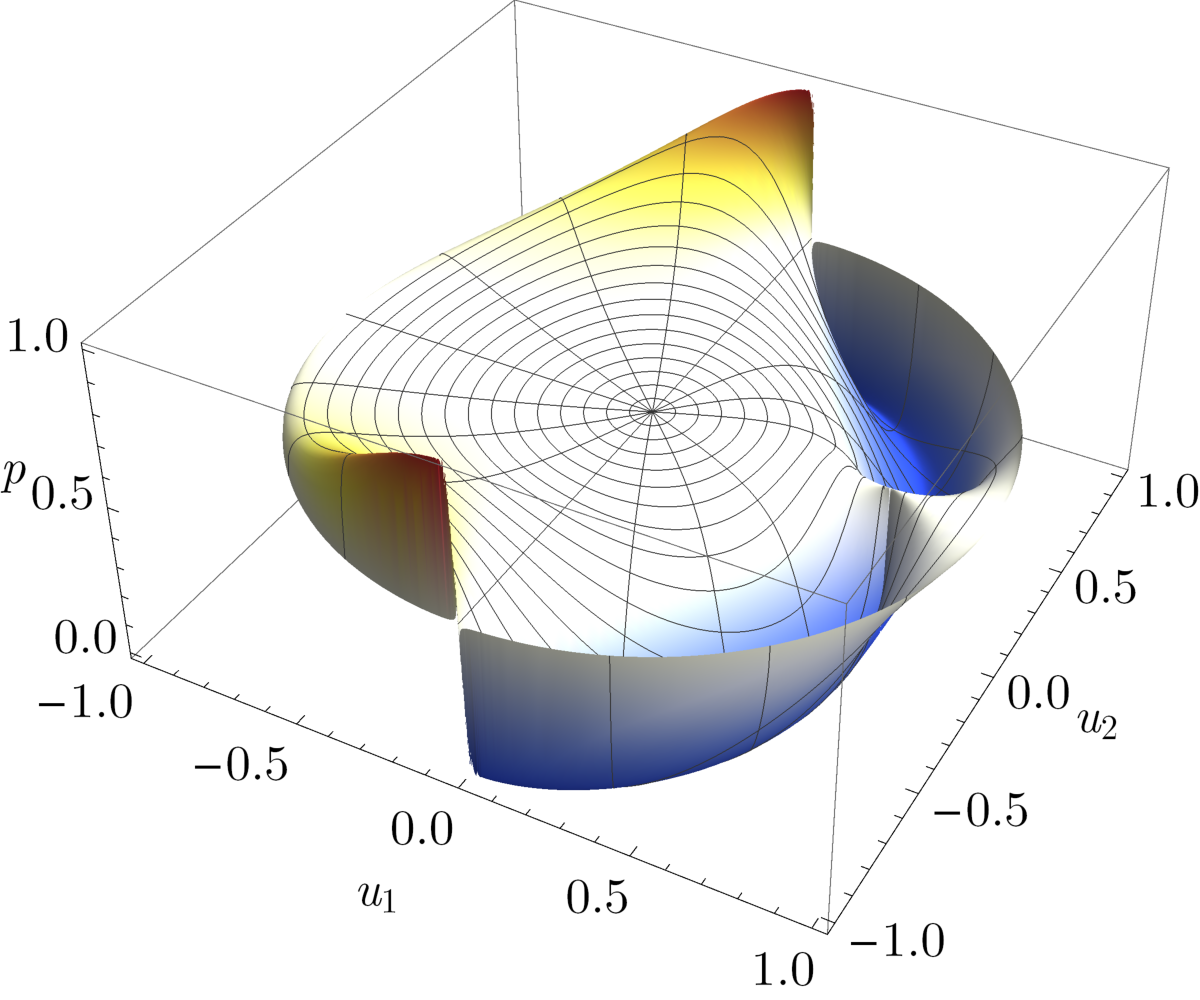
\includegraphics[width=.5\linewidth]{projProbLandscape_2steps_allreal2.pdf}
	\caption{
		Probability given by~\cref{eq:proj_prob_2steps} plotted against $u_1$ and $u_2$, for the special case of $u_1, u_2 \in \RR$.
	}
	\label{fig:proj_prob_landscape_plot3d}
\end{figure}
\begin{figure}[tb]
	\centering
	\begin{tikzpicture}
		\node (img) {\includegraphics[width=.7\columnwidth]%
			{projProbLandscape_2steps_allreal_slices}
		};
		% \node [overlay] (x-axis) at (-.45, -2.4) {\scalebox{1.2}{$u_2$}};
		% \node [overlay] (x-axis) at (-.2, 2.3) {\scalebox{1.2}{$p$}};
	\end{tikzpicture}
	\caption{
		Probability given by~\cref{eq:proj_prob_2steps} plotted against $u_2$, for various choices of $u_1$.
		Each line corresponds to a slice taken from \cref{fig:proj_prob_landscape_plot3d}.}
	\label{fig:proj_prob_landscape_slices}
\end{figure}
\begin{figure}[tb]
	\centering
	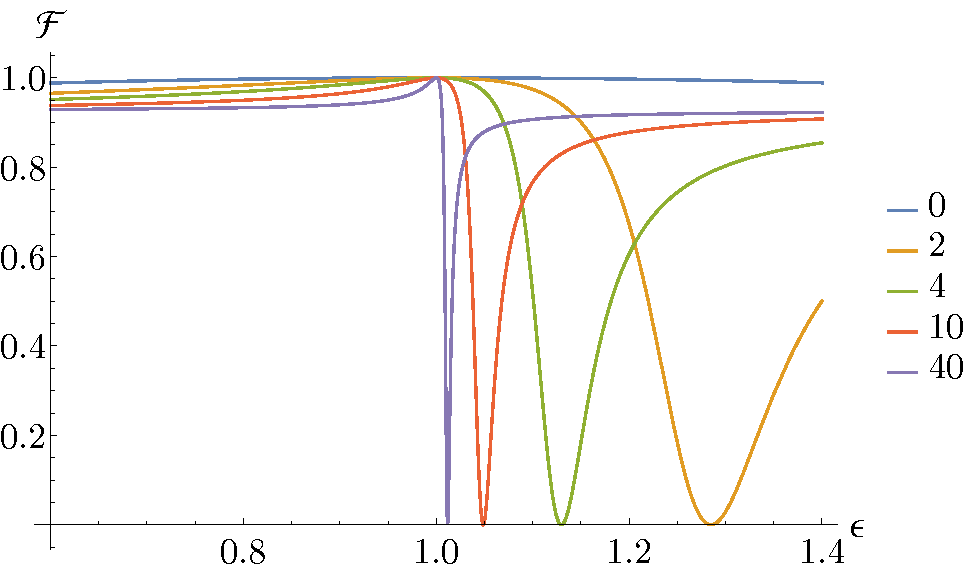
\includegraphics[width=.6\linewidth]{fidelityVsEpsVaryingD_2steps.pdf}
	\caption{
		Fidelity vs a relative change of the value of a coin parameter, for different values of $d_I$.
		Starting from \cref{eq:QWs:state_degenerate_case}, we use as target state the normalised vector
		$\bs u = N (0.5 i, 0.2, 0.5 i)$, and for various values of $d_I$ we compute the coin parameters generating the full state shown in \cref{eq:QWs:state_degenerate_case}.
		We then take a single coin parameter, the parameter $\theta$ in the first step, and substitute it with $\epsilon \theta$, plotting the resulting fidelity between target and generated states as a function of $\epsilon$.
		Larger values of $d_I$ clearly correspond to higher instability.
	}
	\label{fig:fid_vs_eps_varying_d}
\end{figure}

\subsection{Numerical solution of reachability conditions}
\label{sec:QWs:numerical_solution_reachability_conditions}

\tmpHeading{Different numbers of solutions for different numbers of steps}
While, as shown in~\cref{sec:QWs:analytical_sol_2steps}, the $n=2$ case can be fully explored analytically, this is significantly more complicated for larger numbers of steps. Nonetheless,~\cref{eq:QWs:conditions_for_ds} can still be tackled, albeit numerically, for $n=2,3,4,5$.
In this section, we present the results of doing so for a number of random target states sampled uniformly at random.
\Cref{eq:QWs:conditions_for_ds} gives different numbers of solutions for different target states and number of steps:
there is always a single solution for $2$ steps, two or four solutions for $3$ steps, $3, 5, 7$ or $9$ solutions for $4$ steps, and $6, 8, 10, 12, 14$ or $16$ solutions for $5$ steps.

\tmpHeading{Behaviour of projection probabilities}
Different solutions for the same target state correspond to different dynamics before the projection, and therefore different projection probabilities.
This can be seen in~\cref{fig:minmax_probabilities}, where we report maximum and minimum projection probabilities for each randomly generated target state.
These results highlight the advantages of solving~\cref{eq:QWs:conditions_for_ds}: having access to the whole set of solutions, we can choose the most convenient one in terms of projection probability.
Moreover, having access to the various solutions generating a given target state, we can study their stability properties.
As shown in~\cref{fig:stabilities_5steps}, a general trend is that sets of coin parameters associated to smaller projection probabilities are also less stable, in the sense that a small perturbation of a coin parameter can lead to a state significantly different than the target one.

\tmpHeading{Solutions for the special case of fully balanced states}
As an example, we can use this method to generate a balanced superposition over $4$ sites (using therefore $3$ steps): $\ket\phi = (1, 1, 1, 1) / 2$.
This results in two solutions, $\bs d = (-i, 1+i)/2$ and $\bs d = (i, 1 - i)/2$,
corresponding to the full states
\begin{equation}
% \begin{split}
	\frac{1}{2}\Big(
		\ket{1,\uparrow} + 
		(1 \mp i) \ket{2,\uparrow} \pm i \ket{2, \downarrow}
		\pm i \ket{3, \uparrow} + (1 \mp i) \ket{3, \downarrow} +
		\ket{4, \downarrow}
	\Big),
% \end{split}
\end{equation}
which both result in a projection probability over $\ket+$ of 1/4.
The same procedure applied to a balanced superposition over 6 sites (5 steps) results in 6 solutions, 2 of which with real $\bs d$ and projection probability $\simeq 0.145$, and the other 4 with complex $\bs d$ and projections probabilities of 1/6.
It is worth noting that while the projection probabilities over balanced superpositions over $n$ sites seem to vanish with $1/2n$, a simple phase change of an element can radically change this probability.
As an example, again the case of 6 sites, if the target state is instead $\ket\phi \propto (1,1,1,1,1,-1)$ the maximum projection probability becomes $\simeq 0.35$.
The stability of the above solutions for balanced states when a small perturbation is applied to the coin parameters is shown in \cref{fig:stabilities_3and5steps_balanced_target}.


\begin{figure}[]
    \centering
    \begin{minipage}[b]{0.5\textwidth}
        \begin{tikzpicture}
            \node (img) {\includegraphics[width=\columnwidth]%
                {projectionProbabilities_2steps_20000states_histogram40binsProbability}
            };
            \node [overlay] (x-axis) at (3.6, -2.6) {\scalebox{1.2}{$p$}};
            \node [overlay] at (0, 2) {\fbox{2 steps}};
        \end{tikzpicture}
    \end{minipage}%
    \begin{minipage}[b]{0.5\textwidth}
        \begin{tikzpicture}
            \node (img) {\includegraphics[width=\columnwidth]%
                {minMaxProjectionProbabilities_3steps_20000states_histogram40binsProbability}
            };
            \node [overlay] (x-axis) at (4, -2.6) {\scalebox{1.2}{$p$}};
            \node [overlay] at (.2, 2) {\fbox{3 steps}};
        \end{tikzpicture}
    \end{minipage}
    \begin{minipage}[b]{0.5\textwidth}
        \begin{tikzpicture}
            \node (img) {\includegraphics[width=\columnwidth]%
                {minMaxProjectionProbabilities_4steps_20000states_histogram40binsProbability}
            };
            \node [overlay] (x-axis) at (4.2, -2.6) {\scalebox{1.2}{$p$}};
            \node [overlay] at (0, 2) {\fbox{4 steps}};
        \end{tikzpicture}
    \end{minipage}%
    \begin{minipage}[b]{0.5\textwidth}
        \begin{tikzpicture}
            \node (img) {\includegraphics[width=\columnwidth]%
                {minMaxProjectionProbabilities_5steps_6000states_histogram40binsProbability}
            };
            \node [overlay] (x-axis) at (4, -2.6    ) {\scalebox{1.2}{$p$}};
            \node [overlay] at (0, 2) {\fbox{5\,\, steps}};
        \end{tikzpicture}
    \end{minipage}
    \caption{
        Distribution of projection probabilities computed 1) solving~\cref{eq:QWs:conditions_for_ds} for the parameters $d_i$,
        2) computing the projection probabilities associated to each full state given by one such solution set, and
        3) picking the solution set for the $\{d_i\}$ associated to lowest (orange) and highest (blue) projection probabilities.
        The shown data is for the cases of 2, 3, 4 and 5 steps.
        For 2, 3 and 4 steps the data shows the distribution of probabilities from a sample set of 20000 target states, drawn according to the uniform Haar measure over the set of target states.
        For 5 steps only 6000 states were used (being this case much more computationally expensive).
        On the $y$-axis we give the fraction of target states in a given bin.
    }
    \label{fig:minmax_probabilities}
\end{figure}

\FloatBarrier
\subsection{Numerical fidelity maximisation}
\label{sec:QWs:numerical_fid_max}

\tmpHeading{A new method is needed for more than $5$ steps}
Solving numerically~\cref{eq:QWs:conditions_for_ds} for more than $5$ steps is computationally difficult, due to the complexity of the resulting system of equations.
We therefore use a different numerical technique for higher numbers of steps:
we write the fidelity for a given target state as a function of the coin parameters, and find the set of parameters maximizing such fidelity using a numerical optimisation algorithm.
We manage in this way to find solutions for up to $20$ steps much more efficiently than we could have done by directly solving~\cref{eq:QWs:conditions_for_ds}.
% Furthermore, this method eases the study of different final projections, and allows to include the parameters of the projection itself in the optimisation.

\tmpHeading{How we used the optimisation algorithm}
The results of this approach are reported in \cref{fig:prob_histograms_nmaximize}, where we randomly generate a sample of target states, and find through numerical optimisation the set of coin parameters and projections generating them.
It is worth noting that in this procedure we fixed the maximum number of iterations allowed for the maximisation, not the precision with which the final fidelities are to be found.
This is done for the sake of efficiency, as some solutions are found to be more numerically unstable and hard to obtain with very high precisions through numerical optimisation.

\tmpHeading{Results}
As a consequence, as reported in \cref{fig:prob_histograms_nmaximize}, some of the solutions are achieved with relatively low fidelities.
\Cref{fig:prob_histograms_nmaximize} also hints at a correlation between the more unstable solutions and low projection probabilities:
almost all of the solutions that were reached with non-optimal fidelities (that is, fidelity less than 0.99) were also found to correspond to low projection probabilities.
This is consistent with the intuition provided by \cref{fig:stabilities_5steps},
that the lower probability solutions are more unstable with respect to variations of the coin parameters.
\Cref{fig:prob_histograms_nmaximize} shows that in $\sim$90\% (85\%) of the sampled instances we obtain strategies to generate, after 15 (20) steps, states with $p > 0.02$ and $\mathcal F > 0.99$.
% Given the results of~\cref{fig:minmax_probabilities,fig:prob_histograms_nmaximize},
% we believe that this can be sensibly improved by tuning the algorithm.
It is worth noting that --- given the sharp difference between minimum and maximum probabilities reported in \cref{fig:minmax_probabilities}, and the above reasoning substantiated by \cref{fig:fid_vs_eps_varying_d,fig:prob_histograms_nmaximize} ---
% there are strong reasons to believe that even better results can be obtained by properly fine-tuning the optimisation algorithm.
there are strong reasons to believe that almost all target states can be achieved with both high fidelities and probabilities,
by properly fine-tuning the optimisation algorithm.


\section{Conclusions}
\label{sec:QWs:conclusions}

We derived explicit conditions characterising states reachable via time-dependent coined \acp{QW}.
Leveraging this result, we proved that almost all walker states can be probabilistically generated by projecting the coin at the end of the walk.
We found explicit conditions to determine when this is viable, and discussed both analytical and numerical methods to compute the coins generating a target state.
\add{We also analysed the resulting projection probabilities, providing numerical evidence that, at least up to $20$ steps, they are not vanishingly small, and the protocol thus practically feasible.}
Given the ubiquity of \acp{QW}, our approach has the potential to facilitate the engineering of high-dimensional quantum states in a wide range of physical systems.
A possible interesting physical implementation of our protocol uses polarisation and orbital angular momentum of light as physical embodiments of coin and walker states, leveraging the nonlinear optical device known as \emph{q-plate} to implement the controlled-shift operation.
One such implementation will be discussed in~\cref{chapter:experimental_engineering_qudits}.
% Possible future outlooks of our work include exploring the possibility of using two separate quantum walks and leverage 

\add{On top of furthering our understanding of the fundamental structure of QWs, our results suggest a few interesting research directions.
These include exploiting our proposed characterisation of the states producible via QWs to generate states of interest in different applications,
figuring out whether our results can be generalised to more general QW dynamics, \emph{e.g.} ones involving higher-dimensional coins.
Moreover, an interesting venue of future research is figuring out exactly which properties of the QW dynamics make our characterisation possible --- given a dynamics characterised by repeated application of some ``elementary'' operation $\calU_{\bs c}$ parametrised by parameters $\bs c$, when can the full set of output states be characterised as we did for one-dimensional QWs?
An alternative direction of research is exploring what kinds of entangled states can be generated using \emph{pairs} of QWs --- can the single QWs be controlled enough to generate interesting entangled states, or transfer entanglement between coin and walker degrees of freedom?}

\begin{figure}[tbp]
    \centering
    \begin{minipage}[b]{0.5\textwidth}
        \includegraphics[width=\columnwidth]
            {{fidVsParameters_5stepsAnalytical_100thState_prob0.00137738}.pdf}
    \end{minipage}%
    \begin{minipage}[b]{0.5\textwidth}
        \includegraphics[width=\columnwidth]
            {{fidVsParameters_5stepsAnalytical_100thState_prob0.00196137}.pdf}
    \end{minipage}
    \begin{minipage}[b]{0.5\textwidth}
        \includegraphics[width=\columnwidth]
            {{fidVsParameters_5stepsAnalytical_100thState_prob0.00360411}.pdf}
    \end{minipage}%
    \begin{minipage}[b]{0.5\textwidth}
        \includegraphics[width=\columnwidth]
            {{fidVsParameters_5stepsAnalytical_100thState_prob0.00379377}.pdf}
    \end{minipage}
    \begin{minipage}[b]{0.5\textwidth}
        \includegraphics[width=\columnwidth]
            {{fidVsParameters_5stepsAnalytical_100thState_prob0.142292}.pdf}
    \end{minipage}%
    \begin{minipage}[b]{0.5\textwidth}
        \includegraphics[width=\columnwidth]
            {{fidVsParameters_5stepsAnalytical_100thState_prob0.398078}.pdf}
    \end{minipage}
    \begin{tikzpicture}
        \node [overlay] at (-4.65, 0.2) {\scalebox{1}{$\epsilon$}};
        \node [overlay] at (3.77, 0.2) {\scalebox{1}{$\epsilon$}};
    \end{tikzpicture}
    \vspace{0.1cm}
    \caption{
        Behaviour of projection probability of the solutions found solving~\cref{eq:QWs:conditions_for_ds} for the target state $\ket\phi \propto (0.053, -0.078 + 0.603i, -0.524 + 0.189i, -0.302 + 0.363i, 0.182 + 0.099i, 0.042 - 0.224i)$.
        In each of the plots, the final fidelity is plotted against many coin parameters, each time fixing the value of all of them except for one, whose value is changed by an absolute value $\epsilon$ (x-axis).
        The 6 figures correspond to the 6 solutions for this target state, having respectively the projection probabilities:
        $0.0014$ (top left), $0.0020$ (top right),
        $0.0036$ (middle left), $0.0038$ (middle right),
        $0.14$ (bottom left) and $0.398$ (bottom right).
        As clearly illustrated in this case, solutions with low projection probabilities tend to present a higher degree of instability with respect to small changes of the coin parameters.
        A standard parametrisation of $SU(2)$ unitaries is used for the coin operations. The $\theta,\zeta$ notation is in particular the same used in~\cite{chandrashekar2008optimizing}:
        % $U_{\theta,\zeta}=\protect\begin{pmatrix}
        %     \cos\theta & e^{i\zeta}\sin\theta \\
        %     e^{-i\zeta}\sin\theta & -\cos\theta
        % \protect\end{pmatrix}$.
        $\calC_{\theta,\zeta} = \cos(\theta) Z + \sin(\theta)(\cos(\zeta) X - \sin(\zeta) Y)$, with $X,Y,Z$ the Pauli matrices.
        The parameters $\theta_i,\zeta_i$ thus characterise the coin operation at the $i$-th step.
    }
    \label{fig:stabilities_5steps}
\end{figure}

\begin{figure}[]
    \centering
    \begin{minipage}[b]{0.5\textwidth}
        \begin{tikzpicture}
            \node (img) {\includegraphics[width=\columnwidth]%
                {{fidVsParameters_3stepsBalanced_prob0.25}.pdf}
            };
            \node [overlay] (F) at (-3.8, 2.8) {\scalebox{1.2}{$\mathcal F$}};
        \end{tikzpicture}
    \end{minipage}%
    % \begin{minipage}[b]{0.5\textwidth}
    %   \includegraphics[width=\columnwidth]
    %       {{fidVsParameters_3stepsBalanced_prob0.25}.pdf}
    % \end{minipage}%
    \begin{minipage}[b]{0.5\textwidth}
        \begin{tikzpicture}
            \node (img) {\includegraphics[width=\columnwidth]%
                {{fidVsParameters_5stepsBalanced_prob0.667}.pdf}
            };
            \node [overlay] (F) at (-3.8, 2.8) {\scalebox{1.2}{$\mathcal F$}};
        \end{tikzpicture}
    \end{minipage}
    \begin{tikzpicture}
        \node [overlay] at (-4.3, 0.2) {$\epsilon$};
        \node [overlay] at (4.1, 0.2) {$\epsilon$};
    \end{tikzpicture}
    % \begin{minipage}[b]{\columnwidth}
    %   \includegraphics[width=\columnwidth]
    %       {{fidVsParameters_5stepsBalanced_prob0.667}.pdf}
    % \end{minipage}
    \caption{
        Fidelity varying the various coin parameters for 3 (left) and 5 (right) steps, when the target is the completely balanced superposition over 4 and 6 modes, respectively.
        The variation of the coin parameters is here shown as a percentage: the edges of the plots correspond to a variation of 10\% of a single parameter with the others kept fixed at their optimal value.
        The parameters $\theta_i,\xi_i,\zeta_i$ parametrise the coin operations according to
        $\calC_{\theta,\zeta} = \cos(\theta) Z + \sin(\theta)(\cos(\zeta) X - \sin(\zeta) Y)$, with $X,Y,Z$ the Pauli matrices.
        The parameters $\theta_i,\xi_i, \zeta_i$ thus characterise the coin operation at the $i$-th step.
    }
    \label{fig:stabilities_3and5steps_balanced_target}
\end{figure}

\begin{figure}[]
    \centering
    \begin{minipage}[b]{0.5\textwidth}
        \begin{tikzpicture}
            \node (img) {\includegraphics[width=\columnwidth]%
                {probsHistogram_15steps_manyThresholds}
            };
            \node [overlay] (x-axis) at (3.8, -2.8) {\scalebox{1.2}{$p$}};
            \node [overlay] at (0, 2) {\fbox{15 steps}};
        \end{tikzpicture}
    \end{minipage}%
    \begin{minipage}[b]{0.5\textwidth}
        \begin{tikzpicture}
            \node (img) {\includegraphics[width=\columnwidth]%
                {probsHistogram_20steps_manyThresholds}
            };
            \node [overlay] (x-axis) at (4, -2.8) {\scalebox{1.2}{$p$}};
            \node [overlay] at (.2, 2) {\fbox{20 steps}};
        \end{tikzpicture}
    \end{minipage}
    \caption{
        Distribution of projection probabilities for randomly sampled states, computed with the numerical maximisation described in~\cref{sec:QWs:numerical_fid_max}.
        Both plots show the probabilities associated to a set of 3000 target states sampled from the uniform Haar distribution, for 15 and 20 steps.
        The light orange (upper) histograms represent the total number of target states found to correspond to a given range of probability.
        Starting from these datasets, we progressively removed the states that were found to reproduce the target states with fidelity less than $1 - 10^{-t}$, for various values of the threshold $t$.
        Light orange, grey, green, dark orange and purple (from top to bottom) histograms correspond to thresholds of respectively $t = 0, 2, 5, 10, 12$ (higher thresholds correspond to only a handful of states and are therefore omitted).
        This data further suggests a connection between the instability of the found solutions with respect to perturbations of the coin parameters, and the projection probability, as already hinted in \cref{fig:stabilities_5steps}:
        it is harder to find numerically with very good fidelity solutions corresponding to low projection probabilities because of their more unstable nature.
        It is also important to note that the solutions shown here are generally not the optimal ones,
        as the optimisation algorithm only seeks to optimize the final fidelity,
        regardless of the corresponding projection probability.
    }
    \label{fig:prob_histograms_nmaximize}
\end{figure}